\documentclass[12pt]{extarticle}

\usepackage[utf8]{vietnam}
\usepackage{graphicx}
\usepackage{fancyhdr}
\usepackage{parskip}
\usepackage{amssymb}
\usepackage{amsmath}
\usepackage{float}
\usepackage{tikz}
\usepackage{fancybox}
\usetikzlibrary{positioning}
\usepackage[left=3 cm,right=3 cm,top=3cm,bottom=3cm]{geometry}
\usepackage[labelfont=bf]{caption}
\usepackage[hidelinks]{hyperref}
\usepackage{bookmark}
\usepackage{enumitem}
\usepackage[bottom]{footmisc}
\usepackage{multirow}

\pagestyle{fancy}
\renewcommand{\sectionmark}[1]{\markboth{#1}{}} 
\fancyhf{}
\fancyhead[R]{\normalsize{\textit{\leftmark}}}
%\rhead{Phân giải đồng tham chiếu cho đối tượng và thuộc tính trong khai khoáng ý kiến}
\fancyhead[LE,LO]{\thepage}
%\fancyfoot[LE,RO]{\thepage} 
\renewcommand{\headrulewidth}{0.4pt}
%\renewcommand{\footrulewidth}{0.4pt}

\graphicspath{{images/}}

%-----------------SET PARAMS----------------------------------
\tikzset{
  treenode/.style = {shape=rectangle,
                     draw, align=center,
                     top color=white, bottom color=blue!20},
  root/.style     = {treenode, font=\Large, bottom color=red!30},
  env/.style      = {treenode, font=\ttfamily\normalsize},
  dummy/.style    = {circle,draw}
}
%---------------END OF SET PARAMS---------------------------

\begin{document}

%---------------SET FOR DIAGRAM------------------------------
\usetikzlibrary{arrows,chains,positioning,scopes}

\tikzset{
    block/.style={draw,thick,text width=5em,minimum height=6.5em,minimum width=5em,align=center},
    arrow/.style={->, thick}
}

%------------------TITLE PAGE-----------------------------------
\begin{titlepage}

\newcommand{\HRule}{\rule{\linewidth}{0.5mm}} % Defines a new command for the horizontal lines, change thickness here

\center % Center everything on the page
 
%----------------------------------------------------------------------------------------
%	HEADING SECTIONS
%----------------------------------------------------------------------------------------
\begin{flushright}
\end{flushright}
\textsc{\large ĐẠI HỌC BÁCH KHOA THÀNH PHỐ HỒ CHÍ MINH}\\[0.2cm]
\textsc{\Large \scshape khoa khoa học và kỹ thuật máy tính}\\[0.5cm]
\begin{figure}[H] 
\centering
\includegraphics[scale=1.6]{images/logo.jpg}
\end{figure} 

\textsc{\large BÁO CÁO LUẬN VĂN TỐT NGHIỆP}\\[0.2cm] % Minor heading such as course title

%----------------------------------------------------------------------------------------
%	TITLE SECTION
%----------------------------------------------------------------------------------------
\HRule \\[0.4cm]
{ \huge \bfseries Phân giải đồng tham chiếu cho \\ đối tượng và thuộc tính trong\\ khai khoáng ý kiến}\\[0.4cm] % Title of your document
\HRule \\[0.8cm]

%----------------------------------------------------------------------------------------
%	AUTHOR SECTION
%----------------------------------------------------------------------------------------
\begin{flushright}
\begin{minipage}{0.7\textwidth}

\end{minipage}
\end{flushright}

\begin{flushleft} \large
\textbf{Giáo viên hướng dẫn:}\\
GS. TS. Phan Thị Tươi\\[2.0cm]
\end{flushleft}

\begin{flushleft} \large
\textbf{Sinh viên thực hiện:}\\
Nguyễn Đăng Trang - 51203957\\
Nguyễn Trọng Nghĩa - 51202370\\[2cm]
\end{flushleft}

\begin{flushleft} \large
\centering
TP. Hồ Chí Minh, tháng 12 năm 2016
\end{flushleft}

\vfill % Fill the rest of the page with whitespace

\end{titlepage}
%----------------END TITLE PAGE--------------------

\newpage
	\thispagestyle{empty}
	\pdfbookmark{\contentsname}{Mục lục}
	\tableofcontents
	\pagenumbering{arabic}

\newpage
  	\addcontentsline{toc}{section}{Danh sách hình vẽ}
	\listoffigures
	\addcontentsline{toc}{section}{Danh sách bảng}
	\listoftables

\newpage
	\section{Tóm tắt Luận văn}	
		\par Ngôn ngữ của con người chứa đựng nhiều đặc trưng phức tạp và làm cách nào để cho máy tính khai phá có hiệu quả loại dữ liệu này vẫn là một vấn đề lớn. Khai khoáng ý kiến là một lĩnh vực mới phát triển gần đây của Xử lý ngôn ngữ tự nhiên, nó hướng đến việc tìm ra những ý kiến, cảm xúc được biểu đạt qua ngôn ngữ. Bên cạnh đó, bài toán phân giải đồng tham chiếu, mặc dù đã được nghiên cứu rộng rãi nhưng vẫn chỉ được thực hiện trên các loại văn bản chung chung. Các văn bản chứa ý kiến như các bài đánh giá (review), các thảo luận (discussion) về các sản phẩm với các đặc trưng riêng của nó, cung cấp thêm những thông tin nhất định cho việc phân giải đồng tham chiếu trên đó có hiệu quả hơn. Trong Luận văn này, nhóm đề xuất bài toán \textit{Phân giải đồng tham chiếu cho đối tượng và thuộc tính trong khai khoáng ý kiến} với cách tiếp cận theo mô hình Học có giám sát. Dữ liệu được dùng là các văn bản chứa ý kiến bằng ngôn ngữ tiếng Anh. Mô hình do nhóm đề xuất cho kết quả khả quan và gợi mở ra những hướng đi cho việc thực hiện Phân giải đồng tham chiếu cho các văn bản chứa ý kiến trong tiếng Việt.
		
	\section{Giới thiệu đề tài}	
		\par Phân giải đồng tham chiếu (Coreference resolution) là một bài toán quan trọng và được nghiên cứu rộng rãi trong Xử lý ngôn ngữ tự nhiên \cite{mainpaper}. Mục tiêu của bài toán là tìm ra trong văn bản những đề cập (mention) cùng chỉ về một (tập) thực thể trong thế giới thực và gom nhóm chúng thành các chuỗi đồng tham chiếu.?\\
		\textit{Ví dụ}\\
		\textit{Beckham} will visit Vietnam tomorrow. \textit{He} will attend a football event in Saigon.\\
		\textit{Beckham} và \textit{he} trong ví dụ trên cùng chỉ về một thực thể (con người) là cầu thủ bóng đá David Beckham, chúng đồng tham chiếu với nhau.
		\par Tuy nhiên, những nghiên cứu hiện tại về bài toán đồng tham chiếu mới chỉ dừng lại trên các nội dung văn bản tổng quát và không tập trung vàp một loại văn bản cụ thể nào. Mặt khác, cùng với sự phát triển nhanh chóng của thương mại điện tử, người dùng ngày càng có nhu cầu thể hiện ý kiến, cảm xúc của mình đối với sản phẩm. Điều đó được thể hiện qua các bài đánh giá (review) khi mua sắm sản phẩm trực tuyến, các bài đăng (blog post), hay các bài thảo luận trên diễn đàn về sản phẩm (discussion). Trong các văn bản này, người dùng đánh giá về các sản phẩm, cụ thể là họ thể hiện ý kiến đối với đối tượng sản phẩm (object) và các thuộc tính (attribute) của sản phẩm. 
		\par Đối tượng (object) là các thực thể có tên chỉ sản phẩm, mỗi đối tượng bao gồm một tập các bộ phận (component) và một tập các tính chất (feature). Mỗi bộ phận cũng có một tập các bộ phận con và một tập các tính chất của nó. Nói một cách tổng quát, đối tượng có thể được biểu diễn bởi một cây mà nốt gốc chính là đối tượng và các nốt con là các bộ phận, mối liên kết giữa các nốt là các quan hệ thành phần (part-of) \cite{sentiment}. Khi thể hiện ý kiến, người dùng hướng ý kiến đến các nốt của cây và các tính chất của các nốt.\\
		\textit{Ví dụ}\\
		"\textit{The Samsung Galaxy S3} is one of the best phones I've ever used. I absolutely love the phone and \textit{the photo quality} \textit{it} has".\\
		Trong ví dụ trên, người dùng đang đánh giá về đối tượng là chiếc điện thoại \textit{The Samsung Galaxy S3} và thuộc tính của nó là \textit{the photo quality}. Rõ ràng nếu không có phân giải đồng tham chiếu cho đại từ \textit{it}, chúng ta không biết được \textit{it} đang chỉ tới thực thể gì, là đối tượng \textit{The Samsung Galaxy S3} hay thuộc tính \textit{the photo quality}.\\
		\par Hơn nữa, nếu không có phân giải đồng tham chiếu, một lượng thông tin về ý kiến có thể bị mất đi.\\
		\textit{Ví dụ}\\
		"The Galaxy III is pretty cool (1). It's a plastic phone, but it feels solid even though it's very light (2). The screen looks great (3). It is very sharp (4)".
		\\Chúng ta có thể biết được người dùng thể hiện ý kiến ở câu (2) và (4). Nhưng nếu không có phép phân giải đồng tham chiếu để xác định các đại từ "it" trong câu (2) cùng chỉ về đối tượng "The Galaxy III" trong câu (1) và "It" trong câu (4) chỉ về thuộc tính "The screen" trong câu (3), chúng ta không thể biết được người dùng đang thể hiện ý kiến trên thực thể nào.
		\par Trong các văn bản có chứa ý kiến, ngoài đối tượng được xác định là các thực thể có tên, thuộc tính được giả định là đã được tìm ra \cite{findfeatures1} \cite{findfeatures2}. Nhiệm vụ của đề tài là tìm xem những từ/cụm từ nào cùng chỉ về đối tượng hoặc thuộc tính.			

	\section{Các công trình liên quan}
		\subsection{Các công trình liên quan đến phân giải đồng tham chiếu nói chung}
			\par Các công trình này có thể được quy vào ba mô hình dựa theo hướng tiếp cận: Mô hình cặp, mô hình hướng thực thể, mô hình xếp hạng. Nếu xét giải thuật được áp dụng vào bài toán hay nói cách khác là cách sử dụng tập dữ liệu, có ba hướng: Học có giám sát và học không giám sát, hệ thống luật (rules-system). 
			Thống nhất một vài khái niệm, kí hiệu:
				\begin{itemize}
					\item{Yêu cầu của bài toán đồng tham chiếu: Tìm tất cả các chuỗi đồng tham chiếu trong một văn bản; trong đó, mỗi chuỗi đồng tham chiếu là tập hợp các cụm danh từ cùng chỉ đến một thực thể trong thực tế. Từ yêu cầu bài toán, ta thấy đây là một bài toán gom cụm.} 
					\item{Nhóm sử dụng khái niệm "cặp" để nói đến cặp gồm hai cụm danh từ. Kí hiệu cặp (NP1, NP2) được hiểu gồm cụm danh từ NP1 và NP2. Trong đó NP1 xuất hiện trước NP2 trong văn bản, NP1 được gọi là tiền từ và NP2 được gọi là hậu từ.}
					\item{Ta gọi hai cụm danh từ cùng chỉ đến một thực thể là đồng tham chiếu với nhau và chúng nằm trong cùng một chuỗi đồng tham chiếu. Cặp đồng tham chiếu nếu hai cụm danh từ đồng tham chiếu với nhau và cặp không đồng tham chiếu nếu hai cụm danh từ không đồng tham chiếu.}
				\end{itemize}
			\par \textit{Nếu phân loại theo cách tiếp cận, có ba mô hình như sau}
			\subsubsection*{Mô hình cặp (Mention pair)}
				\begin{figure}[H]
					\centering
					% Author: Rasmus Pank Roulund
% \documentclass{minimal}
% \usepackage{tikz}
% \usepackage[utf8]{vietnam}

% \begin{document}
% \usetikzlibrary{arrows,chains,positioning,scopes}

\tikzset{
    block/.style={draw,thick,text width=5em,minimum height=6.5em,minimum width=5em,align=center},
    arrow/.style={->, thick}
}
\begin{tikzpicture}
  {[start chain]
      \node[block,on chain] (N1) {Tập hợp các cụm danh từ};
      \node[block,on chain,join=by {arrow},right=1cm of N1] (N2) {Tạo tập các cặp cụm danh từ};
      \node[block,on chain,join=by {arrow},right=1cm of N2] (N3) {Phân loại các cặp cụm danh từ};
      \node[block,on chain,join=by {arrow},right=1cm of N3] (N4) {Kết hợp những cặp được phân loại đồng tham chiếu};
      \node[block,on chain,join=by {arrow},right=1cm of N4] (N5) {Các chuỗi đồng tham chiếu};
    }
      
  \end{tikzpicture}
% \end{document}
					\caption{Mô hình cặp}
				\end{figure}
				\par Ý tưởng:  Xác định các cặp đồng tham chiếu, sau đó kết hợp các cặp đồng tham chiếu tìm được thành chuối đồng tham chiếu. Bài toán trở thành bài toán phân loại, phân loại tích cực nếu cặp đồng tham chiếu và tiêu cực nếu cặp không đồng tham chiếu.
				\par Tập hợp các NPs $\rightarrow$ tạo tập các cặp chứa 2 NPs có thể có $\rightarrow$ Xác định 2 NPs trong mỗi cặp có đồng tham chiếu $\rightarrow$ Kết hợp kết quả từ tất cả các cặp $\rightarrow$ Các cụm chứa các NPs đồng tham chiếu. (Trình bày mô hình ý tưởng)
				\par Theo như mô hình trình bày ý tưởng từ hình vẽ, mỗi tác giả sẽ có một cách riêng khi thực hiện các bước:
				\begin{itemize}
					\item{Tạo tập các cặp.}
					\item{Tạo tập thuộc  tính để phân loại một cặp là đồng tham chiếu hay không.}
					\item{Cách kết hợp kết quả từ các cặp thu được để tạo ra chuỗi đồng tham chiếu.}
				\end{itemize}
				\par Dưới đây nhóm trình bày cụ thể hơn về các bước trên:
				\begin{itemize}
					\item{Xác định cặp có đồng tham chiếu: 
						\\Để xác định 2 NPs có đồng tham chiếu với nhau hay không, ta cần phải dựa vào tập thuộc tính được tạo ra từ 2 NPs đó. Tập thuộc tính được tạo ra từ đặc điểm cấu trúc cú pháp, ngữ pháp, ngữ nghĩa. Những thuộc tính cơ bản về cú pháp và ngữ nghĩa được trình bày trong bài báo của (Ng và Cardie 2002), tham khảo ở phần Phụ lục A. Những bài báo sau chủ yếu đề xuất thêm những thuộc tính về ngữ nghĩa, ví dụ (Dagan and Itai, 1990; Kehler et al., 2004b; Yang et al., 2005; Haghighi and Klein, 2009…)}
					\item{Cách kết hợp kết quả từ các cặp: 
						\\Từ kết quả xác định đồng tham chiếu của mỗi cặp NPs, ta cần sử dụng giải thuật gom cụm để xác định các cụm chứa các NPs đồng tham chiếu. Dưới đây nhóm trình bày một số giải thuật gom cụm đồng tham chiếu:
						\begin{itemize}
							\item{Giải thuật lựa chọn kết quả gần nhất (Soon 2001): Nếu có các cặp được dự đoán đồng tham chiếu mà hậu từ giống nhau thì Soon chỉ giữ lại cặp đồng tham chiếu mà có khoảng cách từ tiền từ đến hậu từ là gần nhất.}
							\item{Giải thuật lựa chọn kết quả tốt nhất (Ng và Cardie 2002): Nếu có các cặp được dự đoán đồng tham chiếu mà hậu từ giống nhau thì Ng chỉ giữ lại cặp đồng tham chiếu được dự đoán với trọng số cao nhất.}
						\end{itemize}}
						\par Cả hai giải thuật sau đó sử dụng  tính chất bắc cầu để gom cụm. Ví dụ: nếu A đồng tham chiếu B, B đồng tham chiếu C $\rightarrow$ Cụm đồng tham chiếu (A,B,C). Tuy nhiên, nó có vấn đề là: Những cặp có quyết định tích cực được thiên vị hơn những cặp có quyết định tiêu cực. Ví dụ: Mặc dù A và C không đồng tham chiếu, nhưng nếu A và B đồng tham chiếu, B và C đồng tham chiếu thì vẫn đưa ra kết luận cụm đồng tham chiếu (A,B,C).
				\end{itemize}			 
				\par Để giải quyết tình trạng trên thì:
				\par Ưu điểm: Đơn giản, dễ hiện thực.
				\par Nhược điểm:
					\begin{itemize}
						\item{Bài toán được đề ra là bài toán gom cụm, tuy nhiên cách hiện thực lại là kết hợp phân loại trước, gom cụm sau. Kĩ thuật gom cụm ảnh hưởng đến kết quả.}
						\item{Để kiểm tra xem cặp 2 NPs có đồng tham chiếu không, tập thuộc tính chỉ được tạo ra dựa trên 2 NPs đó. Sẽ gặp những trường hợp có những thuộc tính không xác định được. Ví dụ: Mr.Trang has a new phone. Trang also has a new camera. He’s so rich. Trang và He trong trường hợp này  ta không thể xác định chúng có cùng đến một người cùng giới tính hay không. Trong trường hợp đó, nếu ta đã biết Mr.Trang và Trang đồng tham chiếu và sử dụng được thuộc tính từ Mr.Trang, ta có thể suy luận Trang và He có cùng thuộc tính giới tính.}
						\item{Đối với một NP. Ta sẽ xét các cặp từ NP với các tiền từ của nó. Mặc dù có thể dự đoán ra đồng tham chiếu, tuy nhiên ta không thể xác định tiền từ nào phù hợp nhất với một NP vì ta dự đoán độc lập cặp từng tiền từ với NP.}
					\end{itemize}
			\subsubsection*{Mô hình hướng thực thể (Entity-mention)}
				\begin{figure}[H]
					\centering
					% Author: Rasmus Pank Roulund
% \documentclass{minimal}
% \usepackage{tikz}
% \usepackage[utf8]{vietnam}

% \begin{document}
% \usetikzlibrary{arrows,chains,positioning,scopes}

\tikzset{
    block/.style={draw,thick,text width=10em,minimum height=6.5em,minimum width=11em,align=center},
    arrow/.style={->, thick}
}
\begin{tikzpicture}
  {[start chain]
      \node[block,on chain] (N1) {Tập hợp các cụm danh từ};
      \node[block,on chain,join=by {arrow},right=1cm of N1] (N2) {Xem mỗi cụm danh từ là một chuỗi đồng tham chiếu};
      \node[block,on chain,join=by {arrow},right=1cm of N2] (N3) {Tạo các cặp chứa hai chuỗi đồng tham chiếu};
      \node[block,on chain,join=by {arrow},below=1cm of N3] (N4) {Phân loại các cặp đã tạo};
      \node[block,on chain,join=by {arrow},left=1cm of N4] (N5) {Nếu cặp nào được phân loại đồng tham chiếu, gộp hai chuỗi của cặp đó làm một};
      \node[block,on chain,join=by {arrow},left=1cm of N5] (N6) {Các chuỗi đồng tham chiếu};      
    }
      
  \end{tikzpicture}
% \end{document}
					\caption{Mô hình hướng thực thể}
				\end{figure}
				\par Ý tưởng: Xác định xem một cụm danh từ có đồng tham chiếu với một chuỗi đồng tham chiếu (thực thể) hay không. Mục đích của mô hình là phân loại liệu cụm danh từ Nk và chuỗi đồng tham chiếu Cj là tích cực hay tiêu cực, đồng nghĩa với Nk có nên được gán vào chuỗi Cj không.
				\par Tập hợp các NPs $\rightarrow$ Xem mỗi NP là một cụm $\rightarrow$ Xét lần lượt các cụm từ trái sang phải $\rightarrow$ Tìm cụm phù hợp nhất nằm trước cụm đang xét và gộp hai cụm đó lại với nhau $\rightarrow$ Một tập hợp các cụm chứa các NPs đồng tham chiếu. (Trình bày một hiện thực điển hình của mô hình)
				Mỗi cụm danh từ Nk và chuỗi đồng tham chiếu Cj có một tập thuộc tính dùng để phân loại. Tập thuộc tính này gồm: các thuộc tính của Nk, các thuộc tính của Nk với Cj. Điểm đặc trưng của mô hình thực thể và cụm danh từ chính là tập thuộc tính của Nk với Cj. Để xác định một thuộc tính giữa Nk với Cj, ta xét thuộc tính đó giữa Nk với các cụm danh từ trong Cj, từ đó tổng hợp lại. Ví dụ: Để kiểm tra NUMBER AGREEMENT xem Nk có cùng ngôi với Cj không, trước tiên ta kiểm tra lần lược Nk có cùng ngôi với các cụm danh từ trong Cj không. Sau đó ta tổng hợp lại kết quả bằng một vài cách như: NUMBER AGREEMENT là YES nếu Nk cùng ngôi với tất các các NPs trong Cj, NO trong trường hợp còn lại; hoặc như Lou 2004 hay Yang 2004, 2008 là NUMBER AGREEMENT là YES nếu Nk cùng ngôi với ít nhất một NP trong Cj, NO trong tường hợp còn lại. 
				\par Có nhiều biến thể, hình thức hiện thực mô hình, song vẫn giữ nguyên nét đặc trừng là: xây dựng thuộc tính của chuỗi đồng tham chiếu dựa trên các cụm danh từ của nó. Ví dụ Cullota 2007, để giải quyết bài toán đồng tham chiếu, tác giả xác định xác suất một cụm NPs từ văn bản có phải là một chuỗi đồng tham chiếu, tác giả dựa vào thuộc tính chung của cụm NPs đó. Với thuộc tính X của cụm NPs, X nhận giá trị ALL nếu tất cả các cặp của cụm NPs cùng có thuộc tính X, X nhận giá trị MOST-TRUE nếu đa số các cặp của NPs có cùng thuộc tính X và X nhận giá trị MOST-FALSE nếu đa số các cặp của NPs không có cùng thuộc tính X. 
				\par Ưu điểm: Khắc phục được nhược điểm của mô hình Mention Pair, đó là sử dụng thuộc tính của chuỗi đồng tham chiếu, các NPs trong chuỗi có thể bổ sung thuộc tính cho nhau. Trên lý thuyết thì như vậy, tuy nhiên khi áp dụng vào thực tế thì kết quả cũng không được cải thiện nhiều theo Luo et al. (2004), Yang et al. (2004b; 2008a). Lí do là họ vẫn sử dụng ít thuộc tính của chuỗi đồng tham chiếu.
			\subsubsection*{Mô hình xếp hạng (Ranking mention)}
				\begin{figure}[H]
					\centering
					% Author: Rasmus Pank Roulund
% \documentclass{minimal}
% \usepackage{tikz}
% \usepackage[utf8]{vietnam}

% \begin{document}
% \usetikzlibrary{arrows,chains,positioning,scopes}

\tikzset{
    block/.style={draw,thick,text width=6em,minimum height=10em,minimum width=7em,align=center},
    arrow/.style={->, thick}
}
\begin{tikzpicture}
  {[start chain]
      \node[block,on chain] (N1) {Tập hợp các cụm danh từ};
      \node[block,on chain,join=by {arrow},right=1cm of N1] (N2) {Lọc lại các cụm danh từ có khả năng nằm trong chuỗi đồng tham chiếu};
      \node[block,on chain,join=by {arrow},right=1cm of N2] (N3) {Với một cụm danh từ, so sánh các ứng viên cụm danh từ nằm bên trái của nó};
      \node[block,on chain,join=by {arrow},right=1cm of N3] (N4) {Lựa chọn ứng viên có khả năng đồng tham chiếu cao nhất};
      \node[block,on chain,join=by {arrow},below=1cm of N4] (N5) {Tạo các cặp cụm danh từ đồng tham chiếu};
      \node[block,on chain,join=by {arrow},left=1cm of N5] (N6) {Kết hợp những cặp đồng tham chiếu};
      \node[block,on chain,join=by {arrow},left=1cm of N6] (N7) {Tạo các chuỗi đồng tham chiếu};      
    }
      
  \end{tikzpicture}
% \end{document}
					\caption{Mô hình xếp hạng}
				\end{figure}
				\par Ý tưởng: Xét cụm danh từ NP, so sánh tất cả các cụm danh từ đứng trước NP trong văn bản, tìm xem cụm danh từ nào có khả năng đồng tham chiếu với NP nhất. Ta thấy ý tưởng cũng gần giống với mô hình mention pair, đầu ra của cả hai mô hình là cặp đồng tham chiếu.
				\par Tập hợp các NPs $\rightarrow$ Lọc lại các NP có khả năng nằm trong các cụm đồng tham chiếu $\rightarrow$ Xét lần lượt từng NP từ phải sang trái $\rightarrow$ Tìm NP nằm trước phù hợp nhất với NP đang xét $\rightarrow$ Hai NP đó đồng tham chiếu với nhau $\rightarrow$ Một tập hợp các cặp NP đồng tham chiếu $\rightarrow$ Kết hợp kết quả từ các cặp $\rightarrow$ Các cụm chứa các NPs đồng tham chiếu.
				Với một NPs $\rightarrow$ Xét tất cả ứng viên của nó $\rightarrow$ So sánh các ứng viên đó với nhau xem ứng viên nào phù hợp nhất. Ứng viên phù hợp nhất và cụm danh từ sẽ tạo thành một cụm đồng tham chiếu.
				\par Mô hình xếp hạng được áp dụng vào phân giải đồng tham chiếu lần đầu bởi Connolly et al. (1994; 1997). Cụm danh từ Xk có một tập các tiền ngữ K của nó. Xét các cặp (Xi,Xj,Xk) có thể trong đó Xi và Xj thuộc K, phân loại xem (Xi,Xj,Xk) là tích cực hay tiêu cực, nếu tích cực thì Xi đồng tham chiếu với Xk, nếu tiêu cực thì Xj dồng tham chiếu với Xk. Mô hình được biết đến với các biến thể tournament
				model by Iida et al. (2003) and the twin-candidate model by Yang et al. (2003; 2008b). Áp dụng mô hình trên mỗi cặp hai tiền từ của Nk, tiền từ nào có số lần phân loại đồng tham chiếu với Nk cao nhất thì tiền ngữ đó đồng tham chiếu với Nk.
				\par Ưu điểm: So sánh được giữa các tiền từ của một NP, xem tiền từ nào phù hợp đồng tham chiếu nhất.
				\par Nhược điểm: Phải thực hiện một tác vụ: loại bỏ bớt các cụm danh từ NPs từ văn bản mà không có khả năng nằm trong chuỗi đồng tham chiếu. Bới vì những cụm danh từ được giữ lại chắc chắn sẽ được phân loại nằm trong một chuỗi đồng tham chiếu nào đó. Điều này ảnh hưởng đến kết quả mô hình. Denis and Baldridge (2008) và Rahman and Ng (2009) có đề xuất một tác vụ để thực hiện nhiệm vụ này.					
				\par Một số tác giả kết hợp các mô hình trong 3 mô hình trên lại với nhau, trong đó kể đến Rahman and Ng (2009) kết hợp mô hình entity mention với ranking, mục đích so sánh các chuỗi đồng tham chiếu xem chuỗi nào phù hợp với một cụm danh từ đang xét. Mô hình đã khắc phục được hai điểm yếu của mô hình mention pair và cải thiển được kết quả.
			\par \textit{Nếu phân loại theo mô hình học máy, cũng có ba hướng:}
				\subsubsection*{Giải thuật học có giám sát}
					\par Định nghĩa: Giải thuật học có giám sát là giải thuật sử dụng tập dữ liệu có gán nhãn (đã biết trước kết quả) để học. Hai nhánh giải thuật lớn nằm trong học có giám sát là: giải thuật phân lớp và giải thuật hồi quy.
					\par Giải thuật học có giám sát đầu tiên được áp dụng vào bài toán đồngtham chiếu bởi Connolly et al. (1994). Các tác giả thường chuyển bài toán xác định các chuỗi đồng tham chiếu thành bài toán phân loại, do đó giải thuật phân lớp được áp dụng phổ biến. Có thể kể đến: Soon 2001 sử dụng giải thuật cây quyết định C4.5, Ng và Cardie sử dụng giải thuật RIPPER, Yang 2006 sử dụng giải thuật SVM, Maximum Entropy [Denis \& Baldrige, 07], [Ji et al., 05] –.
					\par Ưu điểm:
					\begin{itemize}
						\item{Hệ thống được học dựa trên tập dữ liệu chuẩn đã được gán nhãn.}
						\item{Có các thư viện có sẵn hỗ trợ hiện thực.}
					\end{itemize}
					\par Nhược điểm: Tốn kém chi phí gán nhãn tập dữ liệu. Cần phải có tập dữ liệu gán nhãn thì giải thuật mới học được. 
				\subsubsection*{Giải thuật học không giám sát}
					\par Định nghĩa: Giải thuật học không giám sát là giải thuật sử dụng tập dữ liệu chưa gán nhãn (chưa biết trước kết quả) để học.
					\par Để khắc phục nhược điểm của giải thuật học có giám sát, giải thuật học không giám sát được áp dụng vào bài toán đồng tham chiếu. Mặc dù được áp dụng sau nhưng hiện tại giải thuật học không giám sát đã đạt được kết quả ngang ngửa với giải thuật có giám sát. Haghighi + Klein 2007 sử dụng giải thuật mạng Bayes phi tham số (nonparametric Bayes). Ng 2008 nhận thấy được điểm yếu của giải thuật Bayes phi tham số nên đã đề xuất sử dụng giải thuật Cực đại hóa kì vọng (Expectation Maximization). Cũng cùng thời điểm đó, Poon và Domigos đề xuất phương pháp học không giám sát dựa trên mạng logic Markov (Markov Logic Network) và khẳng định mô hình cho kết quả cao hơn phương pháp học có giám sát.
					\par Ưu điểm:
					\begin{itemize}
						\item{Khắc phục được nhược điểm của giải thuật học có giám sát. Đó là giải thuật học không giám sát có thể được áp dụng vào bất kỳ lĩnh vực đồng tham chiếu nào, chỉ cần có tập dữ liệu chứ không cần phải gán nhãn.}
						\item{Hệ thống được học dựa trên tập dữ liệu dồi dào.}
					\end{itemize}
					\par Nhược điểm: Các giải thuật học không giám sát được áp dụng vào bài toàn đồng tham chiếu thường phức tạp, tác giả tự hiện thực lại.
				\subsubsection*{Hệ thống luật}
					\begin{figure}
						\centering
						% \documentclass{article}
% \usepackage{tikz}
% \usepackage[utf8]{vietnam}

% \begin{document}
% \usetikzlibrary{arrows,chains,positioning,scopes}

\tikzset{    
    arrow/.style={->, thick},
    block/.style={draw,text width=3.5em,minimum height=5em,minimum width=4em,align=center}
}

\begin{tikzpicture}[node distance=2.5cm]
        \node [draw] (np) {Phát hiện các cụm danh từ};        
        \node (table) [shape=rectangle,draw, below of=np] {
            \begin{tabular}{c}
                \hline
                Luật 1: Xác định người nói \\ \hline
                Luật 2: Trùng chuỗi \\ \hline
                . \\ \hline
                . \\ \hline
                . \\ \hline                
                Luật 10: Đại từ giống nhau \\ \hline
            \end{tabular}
        };
        \node [draw, below of=table] (coref) {Các chuỗi đồng tham chiếu};
        \node [above left = 1cm of table] (top_left){};
        \node [below left = 1cm of table] (bottom_left){};
        \node [above right = 1cm of table] (top_right){};
        \node [below right = 1cm of table] (bottom_right){};
        \draw [arrow] (table) -- (coref);
        \draw [arrow] (np) -- (table);        
        \path [draw,arrow] (top_left) --node{}(bottom_left) node [block,pos=0.5,left=0.5cm,font=\footnotesize] {Độ chính xác (Precision) giảm dần};
        \path [draw,arrow] (top_right) --node{}(bottom_right) node [block,pos=0.5,right=0.5cm,font=\footnotesize] {Độ phủ (Recall) tăng dần};        
\end{tikzpicture}

% \end{document}
						\caption{Hệ thống luật}
					\end{figure}
					\par Định nghĩa: Tác giả đề xuất ra một tập các luật quy định khi nào tình hai cụm danh từ là đồng tham chiếu với nhau, khi nào thì cụm danh từ được xét được xét đồng tham chiếu với một cụm dựa trên kinh nghiệm thực tế thu thập được.
					\par Mô hình này được biết đến đầu tiên bởi Baldwin’s 1995. Ý tường tác giả là kết hợp tập các luật có độ chính xác cao theo một thứ tự hợp lý để thu được độ phủ chấp nhận được. Sau đó có nhiều tác giả cũng hiện thực phương pháp này dưới những tên gọi khác nhau như: Brown 1993, Collins + Singer 1999, Spitkovsky 2010. Mô hình gần nhất áp dụng hệ thống luật và đưa lại kết quả cao nhất là Lee, Chang 2012. Trong bài báo, tác giả đề xuất một tập gồm 10 luật, các luật này được sắp xếp có thứ tự dựa vào kết quả độ chính xác (precion) và độ phủ(recall) mà mỗi luật mang lại cho hệ thống. Luật càng đứng trước thì độ chính xác càng cao, luật càng đứng sau thì độ chính xác càng thấp và độ phủ mang lại càng cao. Dữ liệu văn bản sau khi trích xuất ra được các cụm danh từ NPs, các cụm danh từ này lần lượt được kiểm tra với từng luật để tìm đồng tham chiếu, kết quả đầu ra của luật trước là đầu vào của luật sau. Kết quả đầu ra của luật cuối cùng cũng chính là kết quả của hệ thống các luật. Không chỉ áp dụng hệ thống luật, tác giả còn kết hợp với mô hình hướng thực thể (một cách hiểu khác của mô hình thực thể- cụm danh từ) để cải tiến kết quả bài toán.					
					\par Lấy ví dụ về luật số 1 của hệ thống: Nếu người nói là "I" thì từ "my" trong câu nói của người đó sẽ đồng tham chiếu với "I". Ví dụ: < I said "my phone is broken" >, câu văn trên khi đi qua luật số 1 sẽ cho ra kết quả là "I" và "my" đồng tham chiếu.

		\subsection{Các công trình liên quan đến phân giải đồng tham chiếu cho các văn bản chứa ý kiến}
			\par Mỗi lĩnh vực trong thực tế có một đặc điểm dữ liệu riêng. Nếu sử dụng mô hình đồng tham chiếu trên tập dữ liệu chung chung, các đặc điểm chung chung vào một lĩnh vực cụ thể thì kết quả không cao. Xuất phát từ vấn đề đó, những bài toán đồng tham chiếu trên một lĩnh vực cụ thể đang ngày càng gia tăng. Mô hình đồng tham chiếu trong lĩnh vực khai khoáng ý kiến đã được nghiên cứu, tuy nhiên vẫn rất ít. Hai công trình được biết đến nhiều nhất là Stoyanov và Cardie 2006 và Ding + Liu 2010. Stoyanov thực hiện đồng tham chiếu tìm chuỗi đồng tham chiếu cùng chỉ đến một cá nhân, tổ chức trong những bài đánh giá (review) chứa ý kiến.  Trong khi đó, Ding + Liu thực hiện đồng tham chiếu cho đối tượng và thuộc tính. Trong công trình của mình, Liu sử dụng mô hình cặp (mention pair), sử dụng cây quyết định dựa trên tập thuộc tính của Soon 2001 và một số thuộc tính mới liên quan đến cảm xúc và ý kiến mà tác giả đề xuất. Bài báo của Liu là nền tảng để nhóm thực hiện đề tài luận văn.		

	\section{Kiến thức nền tảng}
		\subsection{Bài toán phân giải đồng tham chiếu}
			\label{coref_problem}
			\subsubsection*{Định nghĩa}
				Phân giải đồng tham chiếu trong văn bản là tìm ra trong văn bản những đề cập (mention) cùng chỉ về một (tập) thực thể (con người, sự vật, sự việc, …) hoặc khái niệm trong thế giới thực. Những đề cập (\textit{mention}) này có thể là các từ/cụm từ hoặc các mệnh đề nhưng thông thường là các từ/cụm từ, mà cụ thể hơn là các danh từ/cụm danh từ. Để thống nhất, nhóm dùng khái niệm \textit{mention} trong Luận văn này.
			\subsubsection*{Các quan hệ đồng tham chiếu}		
				Joseph F. McCarthy trong \cite{corefdef} đã chia các quan hệ đồng tham chiếu thành 3 loại: 
				\begin{itemize}
					\item{Quan hệ đồng nhất (Identity): Hai \textit{mention} cùng đề cập tới một thực thể thống nhất\\
					Ví dụ: The iPhone is beautiful. It also works perfectly.
					"The iPhone" và "It" chỉ về một thực thể là một chiếc điện thoại.}
					\item{Quan hệ tập con-tập cha (Subset-superset): Một \textit{mention} nói về tập hợp của các thực thể, một \textit{mention} nói về một thành phần trong tập hợp trên.\\
					Ví dụ: The Nokia and the Samsung are both beautiful. They also work well.\\
					"They" cùng với "The Nokia" và "the Samsung" tham gia vào mối quan hệ tập con-tập cha. Nói một cách khác, "They" chỉ về tập hợp "The Nokia" và "the Samsung", "The Nokia" có mối quan hệ đồng tham chiếu tập con-tập cha với "They", tương tự như "the Samsung".}
					\item{Quan hệ cụ thể-tổng quát (General-Specific): Một \textit{mention} chỉ về một lớp tổng quát, \textit{mention} còn lại chỉ về một thành viên của lớp tổng quát đó.\\
					Ví dụ: I have bought Apple phones yesterday. The iPhone 5 works well and so do the iPhone 6S.\\
					"Apple phones" là một lớp tổng quát. "The iPhone 5" và "the iPhone 6S" là những thành viên của lớp này. 2 cặp "The iPhone 5" – "Apple phones" và ""the iPhone 6S" – "Apple phones" đều có quan hệ đồng tham chiếu kiểu cụ thể-tổng quát.}
				\end{itemize}
			\subsubsection*{Các tính chất của quan hệ đồng tham chiếu}
			Giả sử $M_1$, $M_2$ và $M_3$ là các đề cập trong văn bản.
			\begin{itemize}
				\item{Tính chất phản xạ: Mỗi đề cập ($M_1$, $M_2$, $M_3$) đồng tham chiếu với chính nó.}
				\item{Tính chất đối xứng: Nếu đề cập $M_1$ đồng tham chiếu với $M_2$ thì $M_2$ đồng tham chiếu với $M_1$.}
				\item{Tính chất bắc cầu: Nếu đề cập $M_1$ đồng tham chiếu với $M_2$ và $M_2$ đồng tham chiếu với $M_3$ thì $M_1$ đồng tham chiếu với $M_3$.}
			\end{itemize}
		\subsection{Khai khoáng ý kiến}
			\subsubsection*{Khái quát}
				\par Khai khoáng ý kiến (Sentiment Analysis hay Opinion Mining) trong Xử lý ngôn ngữ tự nhiên là lĩnh vực liên quan đến việc tìm ra những ý kiến, cảm xúc được diễn đạt qua văn bản. Một ý kiến gồm có các thành phần: chủ thể ý kiến (holder), đối tượng (target) và mức độ (orientation) – có thể là tích cực (positive), tiêu cực (negative), trung tính (neutral) hoặc nằm trong một thang đo mức độ (1,2,3,4,5).
				\par Đối tượng (o) là một thực thể chỉ sản phẩm, người, tổ chức, sự kiện, ... Nó có thể được mô hình hóa như sau:\\				
				Đối tượng o gồm một tập các thuộc tính F = \{$f_1$, $f_2$, $f_3$, …\} gồm cả o cũng là một thuộc tính đặc biệt (tổng quát – general). Mỗi thuộc tính fi thuộc F được diễn đạt bằng một hoặc nhiều từ/cụm từ ở trong văn bản (gọi là các synonyms của thuộc tính).
				\par Một văn bản chứa ý kiến (d) chứa một tập các đối tượng O = \{$o_1$, $o_2$, $o_3$, ...\}. Ý kiến được các chủ thể (holder) H = {$h_1$, $h_2$, $h_3$, ...} thể hiện lên mỗi đối tượng và lên các thuộc tính của đối tượng. 
				\par Các nghiên cứu về Khai khoáng ý kiến được thực hiện trên 3 cấp độ \cite{sentiment}:
				\begin{itemize}
					\item{Cấp độ văn bản (Document Level): Xác định thiên hướng ý kiến cho toàn bộ văn bản, với giả định rằng văn bản đó thể hiện ý kiến cho một đối tượng nhất định và từ một chủ thể (holder) nhất định.}		
					\item{Cấp độ câu (Sentence Level): Xác định thiên hướng ý kiến cho một câu, thông thường câu đó cũng được giả định là đang thể hiện ý kiến đối với một đối tượng/thuộc tính (target) nhất định và từ một chủ thể nhất định.}
					\item{Cấp độ thuộc tính (Feature-Based): Các văn bản có chứa ý kiến thường đề cập đến đối tượng và các thuộc tính của nó. Ở cấp độ này, mục tiêu hướng tới là tìm ra thiên hướng ý kiến gắn với các thuộc tính hoặc chính bản thân đối tượng đó.}
				\end{itemize}				

			\subsubsection*{Các từ ngữ chỉ ý kiến}
				\label{ow_section}	
				\par Các từ chỉ ý kiến (Opinion word) là các từ mà bản thân nó mang ý kiến, cảm xúc ở trong câu. Về mặt thiên hướng, chúng được chia thành 2 loại là các từ chỉ ý kiến tích cực (good, amazing, great,… ) và các từ chỉ ý kiến tiêu cực (bad, awful, terrible,…). Bên cạnh các từ đơn, còn có các ngữ (phrase) chỉ ý kiến, đơn cử như "cost someone an arm and a leg". Tập hợp các từ chỉ ý kiến đã được sưu tầm và được sử dụng trong các nghiên cứu \cite{sentiment}, tập hợp này chứa các từ chỉ ý kiến không phụ thuộc lĩnh vực (domain-independent) và không phụ thuộc ngữ cảnh (context-independent).	
				\par Về mặt từ vựng, các từ chỉ ý kiến cũng có thể được chia thành hai dạng là dạng cơ bản (base type) và dạng so sánh (comparative type). Các từ như good, great, bad, ... thuộc dạng cơ bản. Dạng so sánh của chúng như better, best, greater, greatest, worse, worst .. là các dạng so sánh hơn (comparative) và so sánh nhất (supelative) của dạng cơ bản. Khác với dạng cơ bản, dạng so sánh không thể hiện trực tiếp ý kiến (tích cực, tiêu cực) mà thể hiện ý kiến về sự hơn thua giữa các thực thể. Ví dụ: Câu \textit{My Nokia is better than this Samsung} không chỉ ra cụ thể cái nào tốt, cái nào không tốt, nó chỉ thể hiện ý kiến rằng chiếc điện thoại "The Nokia" tốt hơn "this Samsung".
				\par Một vấn đề gặp phải đối với các từ chỉ ý kiến đó là chúng có thể phụ thuộc vào lĩnh vực (domain-dependent). Ví dụ có hai câu "The battery is long" và "The program takes long time to run", "long" đối với "battery" là tích cực nhưng đối với "program" là tiêu cực. Không chỉ vậy, trong cùng lĩnh vực, chúng cũng có thể mang sắc thái khác nhau tùy ngữ cảnh, ví dụ "The battery is long" và "The camera takes long time to focus".	
			\subsubsection*{Khai khoáng ý kiến đối với câu so sánh}
				\label{comparative_section}
				\par Khác với các câu bình thường nơi ý kiến được thể hiện trực tiếp là tích cực hay tiêu cực, ở các câu so sánh, ý kiến được biểu đạt bằng cách thể hiện mức độ hơn, kém, giống nhau trên một khía cạnh nào đó giữa các (tập) đối tượng. Câu so sánh trong tiếng Anh có thể được chia thành 2 nhóm:
				\begin{itemize}
					\item{Nhóm so sánh có cấp độ (Gradable comparison)}	
					\begin{itemize}
						\item{So sánh bằng: Ví dụ: "The Nokia has the same size as this HTC."}					
						\item{So sánh hơn, kém: Ví dụ: "The Nokia has longer battery than this HTC."
							\\hoặc "The Nokia is less expensive than this HTC."}
						\item{So sánh nhất: "The Nokia has the longest battery."}
					\end{itemize}				
					\item{Nhóm so sánh không có cấp độ (Non-gradable comparison)
						\begin{itemize}
						\item{Hai thực thể khác biệt về một đặc trưng nào đó. Ví dụ: "The Nokia has different size to this HTC."}
						\item{Cùng một bộ phận/chức năng nhưng thực thể này dùng cái này, thực thể kia dùng cái khác. Ví dụ: "The Nokia use a SOC from Intel but this HTC use one from Samsung."}
						\item{Thực thể này có bộ phận/chức năng này nhưng thực thể kia không có. Ví dụ: "The Nokia has Bluetooth but this HTC does not."}
						\end{itemize}}					
				\end{itemize}
				\par Hầu hết các câu so sánh trong tiếng Anh đều chứa từ khóa so sánh (ví dụ more, greater, better,…) \cite{sentiment}, chỉ một số lượng nhỏ câu so sánh không chứa. Ví dụ: "I cannot agree with you more". Để phân loại được câu so sánh trong tiếng Anh, ta có thể dựa vào các từ khóa so sánh này.
				\par Trong \cite{comparative1}, Jindal và Bing Liu đã tập hợp các từ khóa so sánh và các mẫu so sánh trong tiếng Anh. GS. Bing Liu, trong \cite{sentiment} đã chia các từ khóa so sánh trong tiếng Anh thành 2 nhóm:
				\begin{itemize}
					\item{Nhóm 1:}		
					\begin{itemize}	
						\item{Các tính từ, trạng từ có một âm tiết hoặc hai âm tiết nhưng kết thúc bởi "y": Các từ so sánh được tạo ra bằng cách thêm đuôi -er (so sánh hơn) hoặc -est (so sánh nhất). Ví dụ: better, happier, greater,...}
						\item{Các tính từ, trạng từ so sánh bất quy tắc: worse, worst, best, least, less,...}		
						\item{Các từ so sánh đặc biệt: prefer, superior,...}
					\end{itemize}
					\item{Nhóm 2: Các tính từ, trạng từ có hai âm tiết còn lại. Các từ so sánh được tạo ra bằng cách thêm more/most/less/least trước từ đó. Ví dụ: more beautiful, most beautiful,...}					
				\end{itemize}
				\par Cũng giống như các câu bình thường, câu so sánh cũng có thể chứa ý kiến hoặc không. Đối với các câu so sánh có ý kiến, như đã đề cập ở trên, ý kiến trên câu chỉ thể hiện mức độ ưu tiên (tốt hơn, đẹp hơn, …) trên một khía cạnh nào đó giữa hai (tập) đối tượng. Ví dụ: "The Nokia is less expensive than this HTC". Ví dụ trên so sánh 2 đối tượng "The Nokia" và "this HTC" trên khía cạnh giá, "The Nokia" là đối tượng được ưu tiên (prefered entity) (ít đắt hơn). 
				\par Để xác định được (tập) đối tượng ưu tiên (prefered entity(s)) trong câu so sánh, phương pháp phân tích dựa trên từ vựng (lexicon-based) có thể được sử dụng. Phương pháp này dựa trên tập các từ chỉ ý kiến (opinion word).
				\begin{itemize}
				\item{Dạng 1: Các từ chỉ ý kiến không phụ thuộc ngữ cảnh (context independent)
					\begin{itemize}
						\item{Đối với các từ so sánh thuộc nhóm 1, ví dụ "better", "worse",… ý kiến được xác định trực tiếp dựa trên ý kiến của từ khóa, ví dụ "better" là tích cực, "worse" là tiêu cực.}
						\item{Đối với các từ so sánh thuộc nhóm 2, cũng có thể dễ dàng dùng các luật sau để tìm ra (tập) đối tượng được ưu tiên.				
							\\<Increasing Comparative> Negative $\rightarrow$ Negative Comparative Opinion
							\\<Increasing Comparative> Positive $\rightarrow$ Positive Comparative Opinion
							\\<Decreasing Comparative> Negative $\rightarrow$ Positive Comparative Opinion
							\\<Decreasing Comparative> Positive $\rightarrow$ Negative Comparative Opinion
							\\Trong đó Negative là từ chỉ ý kiến tiêu cực, Positive là từ chỉ ý kiến tích cực. Increasing Comparative là more, Decreasing Comparative là less.}
					\end{itemize}}
				\item{Dạng 2: Các từ chỉ ý kiến phụ thuộc ngữ cảnh (context dependent). Ví dụ: "The Nokia has longer battery than this HTC". Nếu không có ngữ cảnh "longer battery", ta không thể biết được từ so sánh ở đây "longer" mang nghĩa so sánh tích cực hay tiêu cực để từ đó xác định được đối tượng ưu tiên. Một phương pháp để giải quyết cho trường hợp này được chỉ ra ở \cite{comparative2}.}
				\end{itemize}
		\subsection{Cây quyết định}
			\subsubsection*{Giới thiệu}
				\begin{figure}[H]
					\label{fig:tree}
					\centering
					% Decision tree
% Author: Stefan Kottwitz
% https://www.packtpub.com/hardware-and-creative/latex-cookbook
% \documentclass[border=10pt]{standalone}
% \usepackage{tikz}
% \tikzset{
%   treenode/.style = {shape=rectangle,
%                      draw, align=center,
%                      top color=white, bottom color=blue!20},
%   root/.style     = {treenode, font=\Large, bottom color=red!30},
%   env/.style      = {treenode, font=\ttfamily\normalsize},
%   dummy/.style    = {circle,draw}
% }
% \begin{document}
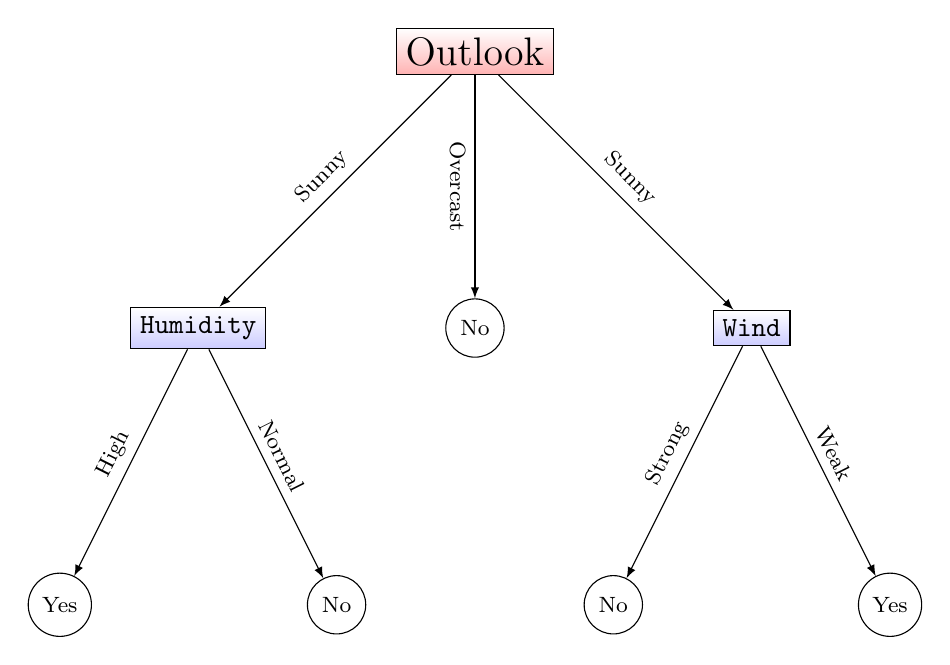
\begin{tikzpicture}
  [
    grow                    = down,
    sibling distance        = 10em,
    level distance          = 10em,
    edge from parent/.style = {draw, -latex},
    every node/.style       = {font=\footnotesize},
    sloped
  ]

\node [root] {Outlook}
    child { node [env] {Humidity}
       child { node [dummy] {Yes}
           edge from parent node [above] {High} }
       child { node [dummy] {No}
            edge from parent node [above] {Normal} }
    edge from parent node [above] {Sunny} }
    child { node [dummy] {No}
      edge from parent node [below] {Overcast} }
    child { node [env] {Wind}
       child { node [dummy] {No}
           edge from parent node [above] {Strong} }
       child { node [dummy] {Yes}
            edge from parent node [above] {Weak} }
    edge from parent node [above] {Sunny} };
\end{tikzpicture}
% \end{document}					
					\caption{Cây quyết định phân loại xem những buổi sáng thứ 7 nào sẽ có chơi Quần vợt (PlayTennis) (Tham khảo từ trang 53 của \cite{mltextbook})}
				\end{figure}
				\par Cây quyết định (Decision Tree) là một mô hình học máy có giám sát, trong đó hàm mục tiêu được mô tả bằng một cây quyết định. Cây quyết định cũng có thể được biểu diễn lại dưới dạng một tập các luật giúp dễ đọc, dễ hiểu.
				\par Mỗi nốt của cây biểu diễn một thuộc tính. Mỗi nhánh xuất phát từ nốt đó thể hiện giá trị của thuộc tính đó. Một mẫu được phân loại trên cây quyết định bằng cách duyệt nó trên cây, bắt đầu từ gốc cho đến khi gặp giá trị phân loại (lá). 
				Cây quyết định ở Hình \ref{fig:tree} xét xem thử những buổi sáng thứ 7 nào sẽ có chơi quần vợt dựa trên các thuộc tính Outlook, Temperature, Humidity, Wind.
				\\Ví dụ mẫu (Outlook = Sunny, Temperature = Cold, Humidity = High, Wind = Strong) duyệt trên cây sẽ cho ra kết quả phân loại là mẫu âm (No). Cây quyết định này cũng có thể được biểu diễn lại thành luật, là hội của các tuyển:
				\begin{center}
					\begin{tabular}{l}				
						(Outlook = Sunny $\wedge$ Humidity = Normal)
						\\$\lor$ (Outlook = Overcast)
						\\$\lor$ (Outlook = Rain $\wedge$ Wind = Weak)
					\end{tabular}
				\end{center}											
			\subsubsection*{Giải thuật}		
				\par Phần lớn các giải thuật học trên cây quyết định (trong đó ID3 là giải thuật điển hình) đều theo hướng tiếp cận từ trên xuống, dùng giải thuật tham lam tìm kiếm trong không gian của tất cả các kết quả cây quyết định có thể xuất hiện. ID3 là giải thuật học cơ bản trên cây quyết định. Phần lớn các giải thuật học trên cây quyết định đều đi theo hướng tiếp cận của ID3, là sự mở rộng và nâng cấp của nó (trong đó có giải thuật C4.5).			
				\par Trong quá trình xây dựng cây từ trên xuống, ở mỗi bước cần xác định được thuộc tính nào là tốt nhất (được hiểu là thuộc tính phân loại hiệu quả nhất cho các mẫu) để làm gốc cho cây ở thời điểm đó. Sự lựa chọn thuộc tính tốt nhất được thực hiện nhờ vào độ đo \textit{Information Gain}.
				\begin{itemize}
					\item{Entropy: Là một hàm đo mức độ không thuần khiết (impurity) của tập mẫu, được sử dụng trong các giải thuật ID3, C4.5. Đối với các tập mẫu thuần khiết, giả sử tập mẫu gồm toàn mẫu âm hoặc dương (xét tập mẫu nhị phân), entropy sẽ bằng 0. Mặt khác đối với các tập mẫu "hỗn độn nhất", với số lượng mẫu âm và dương bằng nhau, entropy sẽ bằng 1. Giá trị của hàm entropy nói chung nằm trong đoạn [0,1] tùy theo số lượng mẫu của các loại. Ngoài ra, một số hàm đo khác (như Gini) có thể được sử dụng thay thể cho hàm Entropy.

					\begin{itemize}
						\item{Công thức Entropy:
						\\Xét tập S là tập mẫu nhị phân gồm các mẫu dương (+) và các mẫu âm (-). Khi đó:
						\begin{equation}					
						Entropy(S) \equiv -p_{(+)}log_{2}p_{(+)} - p_{(-)}log_{2}p_{(-)}
						\end{equation}}						
						\item{Ví dụ: Tập mẫu S gồm 14 mẫu nhị phân, trong đó có 8 mẫu dương và 6 mẫu âm.\\
						Tần số mẫu dương là: 8/14 \\
						Tần số mẫu dương là: 6/14 \\
					 	Khi đó entropy của tập S là:\\	
					 	\begin{align*}						
							Entropy(S) = -(8/14)log_{2}(8/14) - (6/14)log_{2}(6/14) = 0.985
						\end{align*}		
						}
					\end{itemize}}					
					\item{Information Gain: Là một hàm đo độ giảm entropy của tập mẫu khi phân đoạn nó trên một thuộc tính. Độ giảm entropy (độ giảm sự "không thuần khiết") càng cao thì phép phân đoạn đó càng hiệu quả.
					\begin{itemize}
						\item{Công thức Information Gain:
						\\Cho tập S và thuộc tính A. Khi đó: Information Gain của S trên A là:
						\begin{equation}
							\label{eq:gain}
							Gain(S,A) \equiv Entropy(S) - \sum_{v \in values(A)}\frac{|S_v|}{|S|}Entropy(S_v)
						\end{equation}}
						\item{Ví dụ: Tập mẫu S gồm 14 mẫu nhị phân, trong đó có 8 mẫu dương và 6 mẫu âm. 
						Thuộc tính A có 3 giá trị là A1, A2, A3. Thống kê cho thuộc tính A trên S như sau:
						\begin{table}[H]
							\centering							
							\label{my-label}
							\begin{tabular}{|l|l|l|l|}
							\hline
							             & A = A1 & A = A2 & A = A3 \\ \hline
							Số mẫu dương & 2      & 3      & 4      \\ \hline
							Số mẫu âm    & 2      & 2      & 1      \\ \hline
							\end{tabular}
							\caption{Ví dụ tính Information Gain}
						\end{table}
						$\begin{aligned}							
							Entropy(S) = -(8/14)log_{2}(8/14) - (6/14)log_{2}(6/14) = 0.985				
						\end{aligned}$	
						\\
						$\begin{aligned}							
							Entropy(S_{A_1}) = -(2/4)log_{2}(2/4) - (2/4)log_{2}(2/4) = 1				
						\end{aligned}$	
						\\
						$\begin{aligned}							
							Entropy(S_{A_2}) = -(3/5)log_{2}(3/5) - (2/5)log_{2}(2/5) = 0.970
						\end{aligned}$
						\\
						$\begin{aligned}							
							Entropy(S_{A_3}) = -(4/5)log_{2}(4/5) - (1/5)log_{2}(1/5) = 0.722
						\end{aligned}$	
						\\						
						\begin{align*}							
					    	Gain(S,A) &= Entropy(S) - ((4/14)*Entropy(S_{A_1}) + (5/14)*Entropy(S_{A_2}) \\
					    	&+ (5/14)*Entropy(S_{A_3})) = 0.095					    	
						\end{align*}														
						}						
					\end{itemize}}					
				\end{itemize}
				\begin{figure}[H]
					\centering
					% \documentclass{article}

% \begin{document}
% \begin{figure}
	\noindent\fbox{
	    \parbox{\textwidth}{
	        ID3\textit{(Examples, Targetattribute, Attributes)
			\\Examples are the training examples. Targetattribute is the attribute whose value is to be
			predicted by the tree. Attributes is a list of other attributes that may be tested by the learned
			decision tree. Returns a decision tree that correctly classiJies the given Examples.}
			\begin{itemize}
				\item{Create a \textit{Root} node for the tree}
				\item{If all \textit{Examples} are positive, Return the single-node tree \textit{Root}, with label = +}
				\item{If all \textit{Examples} are negative, Return the single-node tree \textit{Root}, with label = -}
				\item{If \textit{Attributes} is empty, Return the single-node tree \textit{Root}, with label = most common value of \textit{Targetattribute} in \textit{Examples}}
				\item{Otherwise Begin
					\begin{itemize}
						\item{A $\gets$ the attribute from \textit{Attributes} that best* classifies \textit{Examples}}
						\item{The decision attribute for \textit{Root} $\gets$ A}
						\item{For each possible value, $v_i$, of A,
							\begin{itemize}
							\item{Add a new tree branch below \textit{Root}, corresponding to the test A = $v_i$}
							\item{Let \textit{$Examples_{v_i}$} be the subset of Examples that have value $v_i$ for A}
							\item{If \textit{$Examples_{v_i}$} is empty
								\begin{itemize}
									\item{Then below this new branch add a leaf node with label = most common value of \textit{Targetattribute} in \textit{Examples}}
									\item{Else below this new branch add the subtree ID3(\textit{$Examples_{v_i}$ (Targetattribute, Attributes - \{A\}})}
								\end{itemize}}
							\end{itemize}}
					\end{itemize}}			
				\item{End}
				\item{Return Root}
			\end{itemize}
			}
		} 	
% \end{figure}
% \end{document}
					* The best attribute is the one with highest information gain, as defined in Equation 
					\ref{eq:gain}
					\caption{Giải thuật ID3 trong cây quyết định (Tham khảo từ trang 59 của \cite{mltextbook})}
					\label{fig:id3}
				\end{figure}
			\subsubsection*{Vấn đề Quá vừa dữ liệu}
				\par Giải thuật ở Hình \ref{fig:id3} là hợp lý trong một số trường hợp, nhưng thực tế nó có thể dẫn đến hiện tượng \textit{Quá vừa dữ liệu (Overfitting data)}. Điều này xảy ra là bởi vì giải thuật này chỉ cố gắng xây dựng cây đủ để phân loại đúng tập huấn luyện, \textit{Quá vừa dữ liệu} sẽ xảy ra nếu dữ liệu trong tập huấn luyện bị nhiễu hoặc chứa quá ít mẫu để có thể xấp xỉ đúng hàm mục tiêu.
				\par Một phương pháp phổ biến được sử dụng để giải quyết hiện tượng này là cho phép cây bị \textit{Quá vừa dữ liệu}, nhưng sau đó cắt tỉa (post-pruning). Trong phương pháp này, tập huấn luyện được chia ra làm hai, một tập huấn luyện (training set) và một tập kiểm chứng phép cắt tỉa (validation set). Cây sẽ được xây dựng dựa trên tập huấn luyện trước, có 2 hướng giải quyết vấn đề cắt tỉa:
				\begin{itemize}
				\item{Cắt tỉa giảm lỗi (reduced error pruning): Cân nhắc từng nốt của cây, và thực hiện cắt tỉa cây con có gốc là nốt đó. Cây sau phép cắt tỉa này được đánh giá độ chính xác dựa vào tập kiểm thử, nếu độ chính xác không thấp hơn cây trước phép cắt tỉa thì cho phép cắt tỉa. Việc cắt tỉa được lặp lại với các nốt không làm giảm độ chính xác của cây cho đến khi không còn lựa chọn nào.}
				\item{Cắt tỉa theo luật (rule post-pruning): Đây là phương pháp được sử dụng trong giải thuật C4.5, bao gồm các bước:
					\begin{itemize}
						\item{Xây dựng cây từ tập huấn luyện}
						\item{Chuyển cây thành một tập các luật}
						\item{Cắt tỉa điều kiện (precondition) trong các luật sao cho độ chính xác không giảm (đối với C4.5, tính toán độ chính xác trên toàn bộ tập huấn luyện)}
						\item{Sắp xếp tập các luật cuối cùng (sau khi cắt tỉa xong) theo độ chính xác và sử dụng các luật này để phân loại cho các mẫu mới (unseen data).}
					\end{itemize}}				
				\end{itemize}

	\section{Phương pháp đề xuất}
		\subsection{Nội dung bài toán}
			\par Cho một văn bản chứa ý kiến gồm một tập các đối tượng O = \{$o_1$,$o_2$,$o_3$,...\}. Giả định của bài toán là ý kiến trong văn bản đều từ một chủ thể duy nhất và tập thuộc tính $F_i$ của các đối tượng đã được tìm ra. Mục tiêu của bài toán là tìm các chuỗi đồng tham chiếu đồng nhất (identity) của đối tượng và thuộc tính.
			\begin{itemize}
				\item{Đầu vào: Văn bản có chứa ý kiến.}
				\item{Giả định:
				\begin{itemize}
					\item{Ý kiến trong văn bản đến từ một chủ thể duy nhất.}
					\item{Các \textit{synonyms} của thuộc tính (bao gồm bản thân đối tượng) đã được tìm ra.}
					\item{Quan hệ đồng tham chiếu thuộc dạng đồng nhất (identity).}
				\end{itemize}}
				\item{Đầu ra: Các chuỗi đồng tham chiếu của đối tượng và thuộc tính.}
			\end{itemize}
			\par Ví dụ: Cho văn bản \\
			\par \textit{I don't like where the power button(1) of Lumia 920(2) is. The battery life(3) is rather poor. I charge it(4) every night and still have had it(5) die on my twice in less than a month. Lumia 920(6) takes great pictures(7). The screen(8) is very sharp and it(9) is easy to watch videos(10) on. However, I want to admit the Lumia(11) is by far better than the iPhone(12)! Learn how to use, and it(13)'s amazing!}	
			\begin{itemize}		
			\item{Tập các đối tượng trong văn bản trên (Các cụm danh từ riêng): \{Lumia 920 (2), Lumia 920(6), the Lumia(11), iPhone(12)\}}
			\item{Giả định đã tìm được tập các synonyms thuộc tính trong văn bản trên: \{the power button(1), the battery life(3), pictures(7), the screen(8), videos(10)\}}
			\item{Đầu ra của bài toán là các chuỗi đồng tham chiếu cho đối tượng và thuộc tính:						
				\begin{center}
					\begin{tabular}{l}
						\{the power button(1)\}
						\\\{Lumia 920(2), it(4), it(5), Lumia 920(6), it(13), the Lumia(11)\}
						\\\{the battery life(3)\}
						\\\{pictures(7)\}
						\\\{the screen(8), it(9)\}
						\\\{videos(10)\}
						\\\{iPhone(12)\}
					\end{tabular}
			 	\end{center}}
		 	\end{itemize}
		\subsection{Tổng quan quy trình}
			\begin{figure}[H]
				\centering				
				% Author: Rasmus Pank Roulund
%\documentclass{minimal}
%\usepackage{tikz}
%\usepackage[utf8]{vietnam}

%\begin{document}
\usetikzlibrary{arrows,chains,positioning,scopes}

\tikzset{
    block/.style={draw,text width=4em,minimum height=6.5em,minimum width=4em,align=center},
    arrow/.style={->, thick}
}
\begin{tikzpicture}
  {[start chain]
        \node[block,on chain] (N1) {Thu thập dữ liệu thô};
        \node[block,on chain,join=by {arrow},right=0.7cm of N1] (N2) {Tiền xử lý dữ liệu};
        \node[block,on chain,join=by {arrow},right=0.7cm of N2] (N3) {Trích xuất cụm danh từ};
        \node[block,on chain,join=by {arrow},right=0.7cm of N3] (N4) {Gán nhãn dữ liệu};
       \node[block,on chain,join=by {arrow},below=0.7cm of N4] (N5) {Trích xuất thuộc tính};
       \node[block,on chain,join=by {arrow},left=0.7cm of N5] (N6) {Tạo tập huấn luyện và tập kiểm tra};
       \node[block,on chain,join=by {arrow},left=0.7cm of N6] (N7) {Áp dụng giải thuật học máy};
       \node[block,on chain,join=by {arrow},left=0.7cm of N7] (N8) {Đánh giá};
    }
      
  \end{tikzpicture}
%\end{document}
			\end{figure}
		\subsection{Tiền xử lý dữ liệu}
		\par Dữ liệu thu thập được sẽ được tiền xử lý nhằm giúp giảm sai số cho các bước sau. Bước tiền xử lý đảm bảo đặc tính ngôn ngữ của văn bản không thay đổi. Sau đây trình bày một số thao tác tiền xử lý mà nhóm đã thực hiện:
		\begin{itemize}
			\item{Tiền xử lý các lỗi liên quan đến đặc tính của công cụ Stanford
				\par Ví dụ: \textit{I am very pleased with the phone we received.It is a genuine Samsung S3.} Từ đầu tiên của câu sau phải cách dấu chấm của câu trước ít nhất một khoảng trắng, trong trường hợp như trên, nếu "It" trong câu 2 nằm ngay sau dấu "." của câu trước nó, công cụ sẽ bắt cả 2 thành chỉ 1 câu, làm cho quá trình phân tích cú pháp (parse) ngay sau đó bị sai.}
			\item{Tiền xử lý các lỗi liên quan đến ngữ pháp của văn bản: Một số câu trong dữ liệu thu thập có thể "sai" ngữ pháp (có thể là do văn phạm của người viết review không thực sự chuẩn xác). 
				\par Ví dụ: \textit{Yes it was hard to see the screen in daylight but I don't expect to see a crystal clear picture on a cell phone, they aren't mini laptops folks.} ("Yes" được dùng ở đầu câu không hợp lý, công cụ bắt "Yes it" là cụm danh từ).			
				\par \textit{I had low expectations about this phone, but when I opened it for the first time I knew it was tend to be mine.} ("was tend" sai ngữ pháp)
				\par Những cú pháp văn phạm sai như vậy làm cho công cụ parsing sai. Hiện tại, với việc thực hiện trên một khối lượng dữ liệu khá nhỏ, trong lúc chọn lọc review nhóm cố gắng đọc và tìm ra các review có cấu trúc văn phạm tiếng Anh đúng, hoặc cố gắng sửa các lỗi nhỏ trong câu để câu được hoàn thiện ngữ pháp. Tuy nhiên, nếu áp dụng trên một khối lượng dữ liệu lớn hơn, những lối văn phạm này sẽ gây ảnh hưởng.} 
		\end{itemize}

		\subsection{Trích xuất cụm danh từ}
			\par Như đã đề cập ở mục \ref{coref_problem}, các \textit{mention} trong bài toán đồng tham chiếu thường là các danh từ/cụm danh từ (từ đây gọi chung là cụm danh từ). Mặt khác trong các văn bản chứa ý kiến, các đối tượng và thuộc tính hầu hết cũng đều được thể hiện bằng các cụm danh từ. Do đó, để trích xuất ra các \textit{mention} phục vụ cho các bước tiếp theo, nhóm thực hiện trích xuất các cụm danh từ trong văn bản. Để thực hiện việc này, trước tiên dùng công cụ Stanford \footnote{http://stanfordnlp.github.io/CoreNLP} để gán nhãn từ loại (part-of-speech) cho các từ và tìm các cụm danh từ dựa vào công cụ CRFChunker \cite{crfchunker}. Tập hợp các cụm danh từ được tìm ra gồm ba loại: các cụm danh từ chỉ đối tượng (cụm danh từ riêng), các cụm danh từ chỉ thuộc tính, các cụm danh từ khác.
			\par Trong nhóm các cụm danh từ khác đã được tìm ra, có những cụm danh từ sẽ không được đưa vào bộ phân loại vì chúng không thể chỉ về đối tượng và thuộc tính. Đó là những cụm danh từ:
				\begin{itemize}
					\item{Các cụm danh từ chỉ dùng nói để nói đến con người: Là các cụm danh từ mà HEAD của chúng thuộc về danh sách sau:
					\par \textit{i;me;myself;we;us;ourselves;you;yourself;yourselves;he;him;himself;
					\\she;her;herself;anyone;someone;somebody;everyone;anybody;everybody;nobody;people}}
					\item{Các cụm danh từ dùng để nói về thời gian: Là các cụm danh từ mà HEAD của chúng thuộc về danh sách sau:
					\par \textit{minute;minutes;hour;hours;day;days;week;weeks;month;months;year;years;
					\\january;february;march;april;may;june;july;august;september;october;november;
					\\december;monday;tuesday;wednesday;thursday;friday;saturday;sunday}}
					\item{Các cụm danh từ dùng để nói về số lượng: Là các cụm danh từ mà HEAD của chúng thuộc về danh sách sau:
					\par \textit{lot;lots;number;total;amount;little;much;many;ton;tons;plenty;some;bit;a}}
					\item{Các cụm danh từ chỉ mốc thời gian: 2PM, 4PM, 5 o'clock.}
					\item{Một số cụm danh từ khác: \textit{there}, \textit{oh}, \textit{etc}, ...}					
				\end{itemize}
			\par Nói về khái niệm HEAD. HEAD của một cụm từ là từ chính của cụm từ đó, nó quyết định dạng cú pháp của cụm từ. Đối với cụm danh từ, HEAD thường là danh từ hoặc đại từ. Ví dụ: Cụm danh từ \textit{the next October} có HEAD là từ \textit{October}.
			\par Ví dụ:
				\textit{I love <this phone>! I was debating between <the regular S5> and <the S5 Active phone>, and I'm so glad I chose <the Active>. I've dropped <my phone> some times already and not even <a dent or scratch> on <it>.}
				\\Các cụm từ trong dấu <> là các cụm danh từ được trích xuất và sử dụng cho các bước tiếp theo.
		\subsection{Gán nhãn dữ liệu}
			\par Mục đích của việc gán nhãn dữ liệu là xác định loại của các cụm danh từ, liệu chúng có chỉ đến đối tượng, thuộc tính không và đồng thời nếu có thì biểu diễn sự đồng tham chiếu đó. Do vậy việc tạo tập dữ liệu để hệ thống học và kiểm tra sẽ dễ dàng hơn.
			\par Mỗi cụm danh từ được gán nhãn có dạng <ID,REF,TYPE NP>. Trong đó:
				\begin{itemize}
					\item{ID: là giá trị nguyên dương duy nhất được gán cho mỗi cụm danh từ, dùng để chỉ vị trí của cụm danh từ trong câu.}
					\item{REF: là giá trị ID của cụm danh từ mà cụm danh từ hiện tại đang  tham chiếu đến.}
					\item{TYPE: là giá trị dùng để phân loại cụm danh từ. 
						\begin{itemize}
							\item{TYPE = 0 nếu cụm danh từ là tên đối tượng}
							\item{TYPE = 3 nếu cụm danh từ là thuộc tính}
							\item{TYPE = 1 nếu cụm danh từ không phải chỉ thuộc tính hoặc đối tượng. Cụm danh từ nào có TYPE là 1 thì giá trị REF của nó là 0.}
							\item{TYPE = 2 nếu cụm danh từ dùng để đại diện cho đối tượng, thuộc tính.}
						\end{itemize}}
					\item{ID: là giá trị nguyên dương duy nhất được gán cho mỗi cụm danh từ, dùng để chỉ vị trí của cụm danh từ trong câu.}
					\item{NP: cụm danh từ.}
				\end{itemize}
			\par Ví dụ: Đoạn văn sau đã được gán nhãn
				\\<0,-1,0 The Note 3> is a lot lighter than <1,-1,0 my HTC EVO>. <2,0,2 It>'s very fast and has <3,0,1 so many features> that <4,-1,0 an IPhone5> can't touch. I love <5,-1,3 the camera > and <6,5,2 it> takes <7,-1,3 great pictures>.
				\\Giải thích: 
				\begin{itemize}
					\item{Các cụm danh từ <0,-1,0 The Note 3>, <1,-1,0 my HTC EVO> và <4,-1,0 an IPhone5> là tên đối tượng (TYPE = 0).}
					\item{<3,0,1 so many features> là cụm danh từ mà không chỉ đối tượng hay thuộc tính (TYPE = 1).}
					\item{<2,0,2 It> và <6,5,2 it> là cụm danh từ đại diện cho đối tượng thuộc tính (TYPE = 2). Trong đó: <2,0,2 It> chỉ đối tượng <0,-1,0 The Note 3> vì có REF = 0; <6,5,2 it> chỉ thuộc tính <5,-1,3 the camera> vì có REF = 5.}
					\item{<5,-1,3 the camera > và <7,-1,3 great pictures> là tên thuộc tính (TYPE = 3).}
				\end{itemize} 

		\subsection{Trích xuất thuộc tính}

			\begin{table}[H]
				\centering
				\begin{tabular}{|l|l|l|}
\hline
Nhóm thuộc tính                                                                               & Thuộc tính                                                                           & Giải thích                                                                                                                                                                                                                                   \\ \hline
\multirow{2}{*}{\begin{tabular}[c]{@{}l@{}}Nhóm liên quan \\ khai khoáng ý kiến\end{tabular}} & Tính nhất quán về ý kiến                                                             & \begin{tabular}[c]{@{}l@{}}Bằng 1 nếu tiền từ và hậu từ có\\ cùng thiên hướng ý kiến. \\ Bằng 0 nếu chúng khác về \\ thiên hướng ý kiến. \\ Nếu không xác định được \\ thiên hướngý kiến cho tiền từ \\ hoặc hậu từ thì bằng 2.\end{tabular} \\ \cline{2-3} 
                                                                                              & \begin{tabular}[c]{@{}l@{}}Sự kết hợp giữa thực thể \\ và từ chỉ ý kiến\end{tabular} & \begin{tabular}[c]{@{}l@{}}Bằng 0,1,2,3,4,10 tùy vào \\ xếp hạng PMI\end{tabular}                                                                                                                                                            \\ \hline
\multirow{6}{*}{\begin{tabular}[c]{@{}l@{}}Nhóm liên quan \\ ngữ pháp\end{tabular}}           & Tiền từ là đại từ                                                                    & \begin{tabular}[c]{@{}l@{}}Bằng 1 nếu tiền từ là đại từ, \\ ngược lại bằng 0\end{tabular}                                                                                                                                                    \\ \cline{2-3} 
                                                                                              & Hậu từ là đại từ                                                                     & \begin{tabular}[c]{@{}l@{}}Bằng 1 nếu hậu từ là đại từ, \\ ngược lại bằng 0\end{tabular}                                                                                                                                                     \\ \cline{2-3} 
                                                                                              & Tính thống nhất về số                                                                & \begin{tabular}[c]{@{}l@{}}Bằng 1 nếu tiền từ và hậu từ \\ thống nhất về số (trong ngữ pháp),\\  ngược lại bằng 0\end{tabular}                                                                                                               \\ \cline{2-3} 
                                                                                              & Từ hạn định                                                                          & \begin{tabular}[c]{@{}l@{}}Bằng 1 nếu hậu từ bắt đầu bằng \\ "the", ngược lại bằng 0\end{tabular}                                                                                                                                            \\ \cline{2-3} 
                                                                                              & Từ chỉ trỏ                                                                           & \begin{tabular}[c]{@{}l@{}}Bằng 1 nếu hậu từ bắt đầu bằng \\ "this", "that", "these", those", \\ ngược lại bằng 0\end{tabular}                                                                                                               \\ \cline{2-3} 
                                                                                              & \begin{tabular}[c]{@{}l@{}}Cả tiền từ và hậu từ \\ đều là danh từ riêng\end{tabular} & \begin{tabular}[c]{@{}l@{}}Bằng 1 nếu tiền từ và hậu từ \\ đều là danh từ riêng, ngược lại \\ bằng 0\end{tabular}                                                                                                                            \\ \hline
\begin{tabular}[c]{@{}l@{}}Nhóm liên quan \\ từ vựng\end{tabular}                             & Tương tự về từ vựng                                                                  & \begin{tabular}[c]{@{}l@{}}Tính tương tự về mặt từ vựng \\ (trùng hoặc gần giống nhau)\end{tabular}                                                                                                                                          \\ \hline
\multirow{3}{*}{Khác}                                                                         & Khoảng cách                                                                          & \begin{tabular}[c]{@{}l@{}}Khoảng cách về câu chứa tiền từ \\ và hậu từ. Nếu chúng nằm cùng \\ một câu thì bằng 0\end{tabular}                                                                                                               \\ \cline{2-3} 
                                                                                              & Từ khóa "is" nằm ở giữa                                                              & \begin{tabular}[c]{@{}l@{}}Bằng 1 nếu có "is" không đi kèm \\ với chỉ định so sánh nào nằm ở \\ giữa tiền từ và hậu từ, ngược lại \\ thì bằng 0\end{tabular}                                                                                 \\ \cline{2-3} 
                                                                                              & Từ khóa "has" nằm ở giữa                                                             & \begin{tabular}[c]{@{}l@{}}Bằng 1 nếu có "has" nằm ở giữa \\ tiền từ và hậu từ, ngược lại thì \\ bằng 0\end{tabular}                                                                                                                         \\ \hline
\end{tabular}
				\caption{Các thuộc tính được sử dụng trong hệ thống}
				\label{features_table}
			\end{table}

			\par Giả sử các cặp \textit{mention} là (NP1, NP2). Sau đây trình bày về các thuộc tính được sử dụng trong hệ thống.

			\subsubsection*{Thuộc tính Khoảng cách (DISTANCE)}
				\par \textit{Giải thích:} Là khoảng cách giữa hai cụm danh từ.
				\par \textit{Giá trị:} [0,1,2,3,…]. Nếu hai cụm danh từ nằm trong cùng một câu thì DISTANCE = 0; nếu hai cụm danh từ nằm trong hai câu liền nhau thì DISTANCE = 1; nếu giữa hai cụm danh từ có n câu (không tính hai câu chứa hai cụm danh từ đó và n > 0) thì DISTANCE = n + 1;
 
			\subsubsection*{Thuộc tính NP1 là đại từ (NP1\_PRONOUN)}
				\par \textit{Giải thích:} Là khả năng cụm danh từ NP1 là đại từ
				\par \textit{Giá trị:} [true, false] Thuộc tính nhận giá trị true nếu NP1 là đại từ và ngược lại nhận giá trị false. Đại từ được nhắc đến bao gồm: đại từ phản thân (itself, themselves), tân ngữ (it, them), đại từ sở hữu (its, theirs), đại từ nhân xưng (it, they) và tính từ sở hữu (its, their).

			\subsubsection*{Thuộc tính NP2 là đại từ (NP2\_PRONOUN)}
				\par \textit{Giải thích:} Là khả năng cụm danh từ NP2 là đại từ
				\par \textit{Giá trị:} [true, false]. Thuộc tính nhận giá trị true nếu NP2 là đại từ và ngược lại nhận giá trị false.

			\subsubsection*{Thuộc tính Cụm danh từ giống nhau (STR\_SIMILARITY)}
				\par \textit{Giải thích:} Là sự giống nhau giữa hai cụm danh từ.
				\par \textit{Giá trị:} [true, false]. Thuộc tính nhận giá trị true nếu danh từ chính của hai cụm danh từ giống nhau và nhận giá trị false nếu ngược lại.

			\subsubsection*{Thuộc tính NP2 là cụm danh từ xác định (DEF\_NP2)}
				\par \textit{Giải thích:} Là khả năng cụm danh từ NP2 là cụm danh từ xác định (cụm danh từ có từ bắt đầu là "the"). 
				\par \textit{Giá trị:} [true, false]. Thuộc tính nhận giá trị true nếu NP2 là cụm danh từ xác định và false nếu ngược lại.

			\subsubsection*{Thuộc tính NP2 là cụm danh từ chỉ định (DEM\_NP2)}
				\par \textit{Giải thích:} Là khả năng cụm danh từ NP2 là cụm danh từ xác định (cụm danh từ có từ bắt đầu là "this", "that", "these" hoặc "those"). 
				\par \textit{Giá trị:} [true, false]. Thuộc tính nhận giá trị true nếu NP2 là cụm danh từ chỉ định và false nếu ngược lại.

			\subsubsection*{Thuộc tính Danh từ riêng (PROPER\_NAME)}
				\par \textit{Giải thích:} Là khả năng cả hai cụm danh từ đều là danh từ riêng.
				\par \textit{Giá trị:} [true, false]. Thuộc tính nhận giá trị true nếu cả hai cụm danh từ đều là danh từ riêng và nếu không phải thì nhận giá trị false.
				\par \textit{Phương pháp hiện thực:} Phần dưới đây trình bày cách xác định một cụm danh từ có là Danh từ riêng hay không.				
				\par Một cụm danh từ gồm nhiều từ, thông qua công cụ gán nhãn từ loại (part of speech) của Stanford, biết được nhãn POS được gán với mỗi từ. Nếu nhãn POS của  một từ nào đó trong cụm danh từ là "NNP" hoặc "NNPs" thì cụm danh từ đó là danh từ riêng bởi vì nhãn "NNP" và "NNPS" có nghĩa là danh từ đó là danh từ riêng. Ví dụ: Trong câu "The Galaxy S3 is beautiful.", cụm danh từ "The Galaxy S3" được công cụ gán nhãn từ loại của Stanford  xử lý thành The/DT Galaxy/NNP S3/NNP. "The Galaxy S3" là danh từ riêng vì có có từ Galaxy và từ S3 được gán nhãn NNP.
				\par Tuy nhiên, trên thực tế vẫn có nhiều tên riêng không tuân theo quy luật trên, công cụ của Stanford không xác định được. Ví dụ: "iphone 6", "iPhone 6" hay "The 620",… Những cụm danh từ này công cụ gán nhãn từ loại của Stanford không gán được nhãn "NNP" hay "NNPS". Vì vậy nhóm đề xuất hướng giải quyết:
				\begin{itemize}
					\item{Tạo danh sách chứa các cụm danh từ riêng đặc biệt là \{"iphone", "iphones", "ipod", "ipad", "ipads"\}, nếu cụm danh từ chứa những từ nằm trong danh sách trên thì cụm danh từ đó là danh từ riêng.}
					\item{Những trường có tên riêng là số, ví dụ: "The 620", "my 8110"…, số được công cụ gán nhãn của Stanford gán nhãn là "CD". Nhóm xác định nếu các cụm danh từ có từ cuối cùng được gán nhãn là "CD" và từ đứng trước nó là mạo từ {a, an, the}, đại từ chỉ định {this, that, these, those} hoặc đại từ sở hữu thì cụm danh từ đó là danh từ riêng.}
				\end{itemize}

			\subsubsection*{Thuộc tính Từ chỉ ý kiến (OPINION\_WORD)}
				\par \textit{Giải thích:} Là quan hệ giữa từ chỉ ý kiến của cụm danh từ NP1 với cụm danh từ NP2.
				\par \textit{Giá trị:} [0,1,2,3,4,10]. 
				\par Từ chỉ ý kiến là danh từ, tính từ hoặc trạng từ thường được dùng để đánh giá một thuộc tính, đối tượng (như đã đề cập trong mục \ref{ow_section}). Ví dụ: với câu "This phone is awesome", từ chỉ ý kiến là "awesome".
				\par Xuất phát từ ý tưởng: những từ chỉ ý kiến thường đi kèm với một số đối tượng, thuộc tính nhất định. Nếu từ chỉ ý kiến đi kèm với cụm danh từ NP1 và nó không bao giờ đi kèm với cụm danh từ NP2 thì dễ dàng thấy rằng khả năng NP1 và NP2 đồng tham chiếu với nhau là rất thấp. Ví dụ đoạn review sau: "The phone does not hold a charge long enough to last the day and it’s expensive." Ta thấy "long" thường được đi kèm với cụm danh từ "a charge" và ít khi đi kèm với cụm danh từ "the phone", nên "a charge" không đồng tham chiếu đến "the phone".
				\par \textit{Giải thuật:}
				\\Để xác định mối quan hệ giữa một từ chỉ ý kiến (OW) với một cụm danh từ (NP), nhóm sử dụng giá trị pointwise mutual information (PMI). Nhóm sử dụng một tập dữ liệu T gồm các bài đánh giá, review để xác định mối quan hệ giữa OW và NP. Nhóm sẽ lần lượt tính các giá trị xác suất P(NP), P(OW), P(NP,OW).
				\begin{itemize} 
					\item{P(NP): Xác suất cụm danh từ xuất hiện trong tập dữ liệu T.}
					\item{P(OW): Xác suất từ chỉ ý kiến xuất hiện trong tập dữ liệu T.}
					\item{P(NP,OW): Xác suất cụm danh từ và từ chỉ ý kiến cùng xuất hiện trong một câu trong tập dữ liệu T.}
				\end{itemize}
				\par Để tính xác suất của một từ, trước tiên ta cần đếm số lần xuất hiện của từ trong tập dữ liệu T.
				\begin{itemize}
					\item{P(NP) = NumOfS(NP)/TotalSentences.
					\\Trong đó: NumOfS(P): số câu trong T chứa cụm danh từ NP. TotalSentences là tổng số câu trong tập dữ liệu T.}
					\item{P(OW) tính tương tự P(NP).}
					\item{P(NP,OW) = NumOfS(NP,OW)/TotalSentences. Với NumOfS(NP,OW) là số câu trong tập dữ liệu T chứa đồng thời NP và OW.}
				\end{itemize}
				\par Khi đã có các giá trị P(NP), P(OW), P(NP,OW) cần thiết, ta tính giá trị mối quan hệ giữa OW với NP theo công thức:
				\begin{center}
					PMI(NP,OW) = log(P(NP,OW)/(P(NP)*P(OW)))
				\end{center}
				\par Giá trị PMI không chỉ biểu hiện mối quan hệ giữa một OW và một NP, mà còn cho ta thấy mối quan hệ giữa cụm danh từ mà OW đang nói đến với NP. Do đó, từ giá trị PMI tính được, nhóm tạo thuộc tính mới OPINION\_WORD cho mỗi mẫu để biểu thị mối quan hệ giữa cặp hai cụm danh từ. Dưới đây là cách hiện thực của nhóm: 
				\par Cụm danh từ NP1 có từ chỉ ý kiến đi kèm là OW1. Đầu tiên, nhóm tính giá trị PMI(NPi,OW1) với NPi là các cụm danh từ nằm trước NP1. Kết quả là nhóm thu được danh sách các giá trị PMI. Cụm danh từ NPi nào có giá trị PMI(Npi,OW1) cao nhất thì thuộc tính OPINION\_WORD của mẫu tạo bởi Npi đó và NP1 là 0, cao thứ nhì thì OPINION\_WORD = 1, cao thứ ba thì OPINION\_WORD = 2, cao thứ tư thì OPINION\_WORD = 3, còn lại OPINION\_WORD = 4. Với trường hợp NP1 không có từ chỉ ý kiến kèm theo, hoặc các giá trị P(NP,OW) = 0, P(NP) = 0, P(OW) = 0 thì  các mẫu tạo bởi cặp đó với các từ đứng trước có giá trị thuộc tính OPINION\_WORD = 10. OPINION\_WORD càng nhỏ thể hiện khả năng hai cụm danh từ có quan hệ càng cao, càng có khả năng đồng tham chiếu với nhau.
				\par Ví dụ: "The phone does not hold a charge long enough to last the day and it’s expensive."
				\\Câu trên có 3 cụm danh từ NP1 "the phone", NP2 "a charge", NP3 "it". Từ chỉ ý kiến OW3 "expensive" đi kèm với NP3. Để tính giá trị thuộc tính OPINION\_WORD cho các cặp (NP1,NP3) và (NP2 NP3), trước tiên ta sẽ tính PMI(NP1, OW3) và PMI(NP2, OW3). Sau khi tính toán, thu được PMI(NP2, OW3) nhỏ hơn PMI(NP1, OW3), khi đó OPINION\_WORD(NP1, NP3) = 0, OPINION\_WORD(NP2, NP3) = 1.
				\par Trong trường hợp một NP có nhiều hơn một từ chỉ ý kiến. Quan hệ giữa hai cụm danh từ không còn dựa trên một từ chỉ ý kiến mà phải dựa vào tập từ chỉ ý kiến. Giá trị PMI dùng để xây dựng giá trị thuộc tính OPINION\_WORD bây giờ là giá trị PMI trung bình. Ví dụ NP1 có OW1 và OW2. Quan hệ giữa cụm từ Npi với N1 không còn chỉ dựa vào PMI(NPi,OW1) hoặc PMI(NPi, OW2) mà dựa vào giá trị PMI trung bình của chúng. Ta lần lượt tính giá trị PMI(NPi,OW1) và PMI(NPi, OW2), giá trị PMI của Npi với tập từ ý kiến là:
				PMI(Npi, {OW1, OW2}) = PMI(Npi,OW1) + PMI(Npi, OW2)/ số từ chỉ ý kiến. 
				Ta tạo giá trị OPINION\_WORD như cách đã trình bày ở trên dựa trên các giá trị PMI(Npi, {OW1, OW2}) đã tính được.
				\par \textit{Phương pháp thực hiện:}
				\\Trước khi có thể tính giá trị PMI, nhóm phải hiện thực nhiệm vụ: Xác định từ chỉ ý kiến trong văn bản. Để thực hiện điều này, nhóm chia nhỏ thành hai công đoạn. Đầu tiên, nhóm tìm tất cả những từ chỉ ý kiến có trong văn bản, sau đó, nhóm tìm cụm danh từ mà những từ chỉ ý kiến đó hướng đến. Dưới đậy, nhóm trình bày kĩ hơn về cách hiện thực hai công đoạn.
				\par Xác định từ chỉ ý kiến trong văn bản:
				\\Từ chỉ ý kiến có thể là danh từ, tính từ, trạng từ. Trong đề tài, nhóm chỉ xác định các từ chỉ ý kiến là tính từ và trạng từ. Theo công cụ gán nhãn Stanford: Từ có nhãn "JJ" hoặc "JJS" hoặc "JJR" là tính từ, từ có nhãn "RB" là trạng từ. Để xác định từ chỉ ý kiến có trong văn bản, nhóm chỉ việc đi tìm những từ có nhãn POS là "RB" hoặc "JJS" hoặc "JJ" hoặc "JJR" và những từ đó xuất hiện trong danh sách L chứa những từ chỉ ý kiến. Danh sách L mà nhóm sử dụng tham khảo từ kết quả trong một bài báo của Liu 200? , bài báo thu thập những từ chỉ ý kiến từ các reviews về điện thoại, máy ảnh.
				\par Xác định cụm danh từ tương ứng với mỗi từ chỉ ý kiến:
				\begin{itemize}
					\item{Từ chỉ ý kiến là trạng từ:
					Trạng từ được xác định là chỉ đến cụm danh từ có đặc điểm: cụm danh từ nằm bên trái gần nhất với trạng từ và giữa cụm danh từ và trạng từ tồn tại ít nhất một động từ. Động từ được xác định là từ có nhãn POS là một trong số các nhãn sau: VB, VBD, VBG, VBN, VBP, VBZ. Ví dụ: Trong câu: "It takes a photo quickly". Trạng từ "quickly" chỉ đến cụm danh từ "It".}
					\item{Từ chỉ ý kiến là tính từ: 
					Áp dụng lần lượt các luật sau để xác định cụm danh từ mà tính từ chỉ đến:
						\begin{itemize}
							\item{Nếu tính từ nằm trong một cụm danh từ thì tính từ được xác định chỉ đến cụm danh từ đó. Ví dụ: từ "fast" chỉ đến cụm danh từ "a fast processor".}
							\item{Nếu tính từ nằm trong câu cảm thán (tính từ nằm sau từ "how") thì tính từ chỉ đến cụm danh từ nằm phía sau gần nó nhất. Ví dụ: Trong câu "How beautiful the camera is". Tính từ "beautiful" được xác định chỉ đến cụm danh từ "the camera".}
							\item{Nếu liền phía sau tính từ là một cụm danh từ thì tính từ được xác định chỉ tới cụm danh từ đó. Ví dụ: "The Lumia 920 has a good camera". Tính từ "good" được xác định chỉ đến cụm danh từ liền sau nó là "camera".}
							\item{Tính từ được xác định là chỉ đến cụm danh từ có đặc điểm: cụm danh từ nằm bên trái gần nhất với tính từ và giữa cụm danh từ và tính từ tồn tại ít nhất một động từ. Ví dụ: "The camera is good". Tính từ "good" được xác định chỉ đến cụm danh từ "the camera".}
						\end{itemize}}
				\end{itemize}

			\subsubsection*{Thuộc tính Thống nhất về số (NUMBER\_AGREEMENT)}
				\par \textit{Giải thích:} Hai cụm danh từ cùng mang ý nghĩa số ít hoặc cùng mang ý nghĩa số nhiều thì xác suất chúng đồng tham chiếu là cao hơn trường hợp ngược lại. 
				\par \textit{Giá trị:} [true, false]. Thuộc tính nhận giá trị true nếu cả hai cụm danh từ có cùng "số" và nếu không phải thì nhận giá trị false.
				\par Để trích xuất thuộc tính này, nhóm sử dụng công cụ Stanford để tìm ra HEAD của mỗi cụm danh từ ứng viên và "số" của HEAD được coi là "số" của cụm danh từ chứa nó. Nếu HEAD là danh từ "số" được xác định dựa trên POS Tag của chính nó (NN, NNP cho số ít) và (NNS, NNPS cho số nhiều). Nếu HEAD là đại từ, "số" của nó được gán dựa vào một list các đại từ số nhiều và số ít đã được tổng hợp.
				\par Ví dụ:
				\\"I transfered my old phone to my friend and now consider to buy two new phones. They are both Motorola". Two new phones và they khả năng là đồng tham chiếu vì chúng đều là số nhiều (phones và they số nhiều), trong khi my old phone là số ít do đó nếu bắt cặp nó với they chẳng hạn thì chúng không thể đồng tham chiếu được.				

			\subsubsection*{Thuộc tính Từ khóa "is" nằm ở giữa (IS\_BETWEEN)}
				\par \textit{Giải thích:} Nếu ở giữa 2 cụm danh từ trong câu có từ "is" và nó không đi kèm với bất kỳ chỉ định so sánh nào thì có xác suất để 2 cụm danh từ này đồng tham chiếu. Nếu ở giữa 2 cụm danh từ trong câu có từ "is" và nó có đi kèm với một chỉ định so sánh nào thì có xác suất để 2 cụm danh từ này trỏ tới 2 thực thể/thuộc tính khác nhau.
				\par \textit{Giá trị:} [true, false]. Thuộc tính nhận giá trị true nếu ở giữa 2 cụm danh từ trong câu có từ "is" đồng thời không có chỉ định so sánh nào, ngược lại nhận giá trị false.
				\par Về việc xác định các chỉ định so sánh, các chỉ định so sánh được tìm kiếm bằng cách bắt các từ/cụm từ thuộc các mẫu so sánh phổ biến (đã đề cập ở mục \ref{comparative_section}).
				\par Ví dụ: 
				\\"Nokia 215 is my second phone". "Nokia 215" và "my second phone" khả năng đồng tham chiếu với nhau.
				\\"Overall the K800 is far superior to the W810". "K8100" và "W810" khả năng trỏ tới 2 thực thể khác nhau.

			\subsubsection*{Thuộc tính Từ khóa "has" nằm ở giữa (HAS\_BETWEEN)}
				\par \textit{Giải thích:} Nếu ở giữa 2 cụm danh từ trong câu có từ "has" thì có xác suất để 2 cụm danh từ này trỏ tới 2 đối tượng/thuộc tính khác nhau, giữa chúng có thể là mối quan hệ bộ phận (part-of). 
				\par \textit{Giá trị:} [true, false]. Thuộc tính nhận giá trị true nếu ở giữa 2 cụm danh từ trong câu có từ "has", ngược lại nhận giá trị false.
				\par Ví dụ:
				"My MiPad has a 5MP front camera". My MiPad và a 5MP front camera khả năng trỏ tới 2 thực thể/thuộc tính khác nhau
								
				\par \textit{Phương pháp hiện thực:}
				\\Nếu giữa hai cụm danh từ có chứa từ "has" hoặc "have" hoặc "had" và từ đi kèm sau chúng không phải là "to" hay động từ nhóm 3 (nhãn POS là "VBN") thì thuộc tính HAS\_BETWEEN của cặp hai cụm danh từ là true. Trong những trường hợp còn lại HAS\_BETWEEN bằng false.

			\subsubsection*{Thuộc tính Nhất quán về ý kiến (SENTIMENT\_CONSISTENCY)}
				\par \textit{Giải thích:} Khi người dùng giới thiệu một đối tượng và thể hiện ý kiến đối với nó trong một câu, họ có xu hướng nhắc lại đối tượng đó trong câu tiếp theo và với cùng ý kiến. Hiện tượng này là dễ bắt gặp trong các văn bản chứa ý kiến.
				\par \textit{Giá trị:} [0,1,2]
				\\Nếu NP1 và NP2 cùng thiên hướng ý kiến $\Rightarrow$ 1
				\\Nếu NP1 và NP2 khác thiên hướng ý kiến $\Rightarrow$ 0
				\\Nếu không biết thiên hướng ý kiến trên NP1 hoặc NP2 $\Rightarrow$ 2

				\par (1) Nếu s(i-1) và s(i) đều là câu bình thường 
				\\Giả sử có NP1 ở câu s(i-1) và NP2 ở câu s(i)
				\begin{itemize}
					\item{Nếu thiên hướng ý kiến đối với NP1 và NP2 là giống nhau (cùng tích cực hoặc tiêu cực) thì chúng có khả năng là đồng tham chiếu.}
					\item{Nếu thiên hướng ý kiến đối với NP1 và NP2 là khác nhau, chúng có khả năng là không đồng tham chiếu.}
				\end{itemize}
				(2)	Nếu s(i-1) là câu so sánh (câu so sánh được xác định dựa trên một số luật như câu chứa các chỉ định so sánh tương tự như trong thuộc tính số 10 "is between") và s(i) là câu bình thường
				\begin{itemize}
					\item{Giả sử có NP1 và NP2 ở câu s(i-1) được so sánh với nhau (2 cụm danh từ gần nhất 2 bên chỉ định so sánh) và NP3 là cụm danh từ ở s(i)}
					\item{Dựa vào thiên hướng ý kiến của câu so sánh(i-1), như đã đề cập ở mục \ref{comparative_section} thiên hướng ý kiến của câu so sánh có thể được tìm ra dựa vào từ khóa so sánh. Ví dụ: s(i-1) là một câu so sánh có dạng NP1 is better than NP2, vì better có thiên hướng so sánh tích cực nên ta xác định được đối tượng ưu tiên trong phép so sánh này là NP1. Vì vậy nếu thiên hướng ý kiến đối với NP3 là tích cực thì NP3 có khả năng đồng tham chiếu với NP1, ngược lại nó có khả năng đồng tham chiếu với NP2.
					\\ Ví dụ:
					\\\textit{However, I want to admit Lumia 920 is by far better than the iPhone! Learn how to use, and it's amazing!.} 
					\\Nhờ từ khóa so sánh better, ta xác định được đối tượng ưu tiên là Lumia 920. Ở câu tiếp theo do thiên hướng đối với đại từ it là tích cực (dựa vào từ chỉ ý kiến amazing gắn với nó) nên it có khả năng đang nói tới đối tượng Lumia 920, theo tính chất nhất quán về ý kiến trong ngôn ngữ.
					\\\\\textit{Stylo 2 is a great phone. It is very fast with plenty of storage for apps.}
					\\Câu đầu tiên giới thiệu về đối tượng Stylo2 với thiên hướng tích cực (nhờ vào từ chỉ ý kiến great). Ở câu tiếp theo do thiên hướng đối với đại từ it là tích cực (dựa vào từ chỉ ý kiến fast gắn với nó) nên it có khả năng đang nói tới đối tượng Stylo2, theo tính chất nhất quán về ý kiến trong ngôn ngữ.}
				\end{itemize}
				\par Để xác định được thiên hướng ý kiến đối với 1 cụm danh từ bất kỳ, nhóm sử dụng từ chỉ ý kiến đi kèm với cụm danh từ này. Nếu từ chỉ ý kiến là tích cực/tiêu cực thì tương ứng thiên hướng ý kiến đối với cụm danh từ đó là tích cực/tiêu cực. Nếu không có từ chỉ ý kiến nào đi kèm thì cụm danh từ đó được xác định là không rõ thiên hướng ý kiến.

		\subsection{Tạo bộ phân loại}
			\subsubsection*{Tạo tập huấn luyện}
				\par Giải thuật phân loại nhận đầu vào để học là một tập các mẫu. Một mẫu dùng để học (instance) có dạng: Instance = (<$f_1$,$f_2$,…,$f_n$>, y), trong đó n thể hiện mẫu có n thuộc tính, $f_i$ thể hiện giá trị của thuộc tính thứ i, y thể hiện giá trị phân loại đầu ra của mẫu. Cứ mỗi cặp (NP1, NP2) tạo được một mẫu. 
				\\Từ tập dữ liệu học, ta xác định được danh sách L chứa các cụm danh từ NPs.
				\par Tập mẫu dùng để học (Instances): mọi cặp (NP1, NP2) được tạo ra từ danh sách L và thỏa mãn điều kiện NP1 hoặc NP2 là cụm danh từ chỉ đối tượng/thuộc tính (TYPE = 0 hoặc TYPE = 2 hoặc TYPE = 3). Bởi vì đề tài chỉ thực hiện với mục đích phân giải đồng tham chiếu các đối tượng/thuộc tính nên nhóm không xét trường hợp các cặp (NP1,NP2) mà NP1 và NP2 đều không chỉ đối tượng/thuộc tính (TYPE = 1).
				\\Đặc điểm mỗi mẫu dữ liệu để học:
				\begin{itemize}
					\item{Tập thuộc tính: đã được đề cập ở phần 3.}
					\item{Giá trị phân loại: (NP1, NP2) được gán nhãn phân loại là true nếu:
						\begin{itemize}
							\item{TYPE của NP1 và NP2 là 0 hoặc 2 hoặc 3 (NP1 và NP2 là cụm danh từ chỉ đối tượng hoặc thuộc tính).}
							\item{Giá trị REF của NP2 bằng giá trị REF của NP1 hoặc giá trị REF của NP2 bằng giá trị ID của NP1. (NP1, NP2) nhận giá trị false trong những trường hợp còn lại.}
						\end{itemize}}
				\end{itemize}
				\par Ví dụ: Xem xét đoạn văn bản đã được đánh dấu dưới đây:
				\\I have owned <0,-1,0 the Nokia 6101> since <1,0,1 late October 2005>. I absolutely love <2,0,0 it>! I wouldn't trade <3,2,0 it> for <4,0,1 the world>.
				\\Tập dữ liệu học được xây dựng từ đoạn văn bản trên được trình bày bên dưới:
				\begin{figure}[H] 
					\centering
					\includegraphics{images/examples_train.png}
				\end{figure} 
				\par Thứ tự ý nghĩa của các giá trị trong mỗi mẫu là: ID\_NP1, ID\_NP2, NP1\_PRONOUN, NP2\_PRONOUN, DEF\_NP2, DEM\_NP2, PROPER\_NAME, STR\_MARCH, DISTANCE, NUMBER, IS\_BETWEEN, HAS\_BETWEEN, COMPARATIVE, SENTIMENT, PMI, IS\_NESTED, COREF.
			\subsubsection*{Tạo tập kiểm tra}
				\par Giải thuật phân loại sau khi đã học xong sẽ được áp dụng trên một tập dữ liệu kiểm tra. Nó được áp dụng trên một tập các mẫu. Một mẫu có cấu trúc giống như mẫu dùng để học. Mỗi mẫu (instance) có dạng: Instance = (<$f_1$,$f_2$,…,$f_n$>, y), trong đó n thể hiện mẫu có n thuộc tính, fi thể hiện giá trị của thuộc tính thứ i, y thể hiện giá trị phân loại đầu ra của mẫu. Cứ mỗi cặp (NP1, NP2) tạo được một mẫu. 
				\\Từ tập dữ liệu dùng để kiểm tra, ta xác định được danh sách T chứa các cụm danh từ NPs. Tập mẫu dùng để kiểm tra (Instances): mọi cặp (NP1, NP2) được tạo ra từ danh sách T. Đặc điểm mỗi mẫu dữ liệu để kiểm tra giống với đặc điểm của mẫu dữ liệu dùng để học.
			\subsubsection*{Kiểm chứng chéo}
				\par Kiểm chứng chéo (cross validation) là việc phân nhóm mẫu dữ liệu thành nhiều mẫu con //TODO
				\par Nhóm áp dụng giải thuật k-fold cross validation để học và kiểm tra hệ thống. Bởi vì tập dữ liệu gồm 157 reviews, nhóm lựa chọn k = 5. Tập dữ liệu được chia làm 5 tập, mỗi tập gồm 31-32 reviews. Hệ thống sẽ thực hiện học và kiểm tra 5 lần liên tiếp, kết quả đánh giá hệ thống dựa trên trung bình kết quả của các lần học và kiểm tra. Tại lần học thứ i, hệ thống sử dụng tập thứ i để tạo tập dữ liệu kiểm tra và các tập còn lại để tạo dữ liệu dùng để học.

			\subsubsection*{Áp dụng giải thuật học Cây quyết định}
				\par Các cặp ứng viên được phân loại dựa vào Cây quyết định bằng giải thuật J48 trên Weka \footnote{http://www.cs.waikato.ac.nz/ml/weka}. J48 là sự hiện thực của giải thuật C4.5.
		\subsection{Gom cụm các đồng tham chiếu}	
			\par Dựa vào kết quả phân loại các cặp ứng viên, thực hiện gom cụm đồng tham chiếu							

	\section{Thực nghiệm và đánh giá}
		\subsection{Thực nghiệm}
			\subsubsection*{Chương trình}
				\par Hệ thống được hiện thực bằng ngôn ngữ Java (JDK1.8), dùng tới các thư viện của công cụ Stanford, Weka và code của công cụ CRFChunker. Chương trình được tổ chức thành các gói (package) sau:
				\begin{itemize}
					\item{element: Gói này gồm các lớp (class) lưu thông tin liên quan đến các thành phần trong ngôn ngữ tự nhiên như Review(văn bản), Sentence(câu), NounPhrase(cụm danh từ), Token(thẻ), CorefChain(chuỗi đồng tham chiếu) với các mối quan hệ has-a giữa các lớp.}
					\item{gui: Gói liên quan đến giao diện.}
					\item{process: Gói liên quan đến quá trình trích xuất thuộc tính hoặc gán nhãn dữ liệu.}
					\item{test: Gói liên quan đến việc hiện thực các độ đo chuỗi đồng tham chiếu.}
					\item{util: Gói liên quan đến việc trích xuất các thành phần của ngôn ngữ tự nhiên, dựa vào thư viện của công cụ Stanford, bao gồm cả việc lấy HEAD của các cụm danh từ.}
					\item{weka: Gói liên quan đến việc tạo bộ phân loại dựa trên công cụ Weka, gồm cả việc dùng Cây quyết định.}
				\end{itemize}
				\par Gói công cụ Xử lý ngôn ngữ tự nhiên của Stanford bao gồm các công cụ khác nhau phục vụ cho từng công việc: phân tách các token (tokenize), phân tách câu (ssplit), gán nhãn từ loại (pos), phân tích cú pháp (parse).
			\subsubsection*{Dữ liệu thực nghiệm}

			\subsection{Đánh giá}			
				\subsubsection*{Phương pháp đánh giá}
					\par Từ tính chất bắc cầu: Nếu cặp (A,B) đồng tham chiếu, (B,C) đồng  tham chiếu thì ta có chuỗi đồng tham chiếu gồm A, B, C. Như vậy, từ tập dữ liệu kiểm tra ta có được:
						\begin{itemize}
					 		\item{Tập thực tế S: các chuỗi $S_i$ đồng tham chiếu thực tế. Mỗi cụm $S_i$ có 2 cụm danh từ trở lên.}				
							\item{Tập dự đoán R: các chuỗi $R_i$ đồng tham chiếu mà hệ thống dự đoán. Trong đó mỗi chuỗi phải chứa ít nhất một tên đối tượng hoặc thuộc tính (cụm danh từ trên thực tế có TYPE = 0 hoặc TYPE = 3), nếu không chuỗi đó sẽ bị bỏ đi khỏi tập dự đoán. Mỗi chuỗi $R_i$ có 2 cụm danh từ trở lên.}
						\end{itemize}
					\par Nhóm sử dụng 3 độ đo phổ biến trong bài toán đồng tham chiếu để so sánh tập dự đoán với tập thực tế, đó là: MUC, B3 và CEAF-4.
					\par \textit{MUC SCORE}
					\\Một số khái niệm:
						\begin{itemize}
							\item{$S_i$ = \{A B C D\}: chuỗi đồng tham chiếu $S_i$ chứa 4 cụm danh từ là A, B, C, D.}
							\item{|$S_i$|: số cụm danh từ thuộc chuỗi $S_i$. Ví dụ chuỗi $S_1$ = \{A B C D\} thì |$S_1$| = 4.}
							\item{p($S_i$): tập hợp các cụm $P_j$ của chuỗi $S_i$. Mỗi cụm $P_j$ chứa các cụm danh từ, tối thiểu là một cụm danh từ. Cách tìm $P_j$: $P_j$ = $S_i$ giao $R_i$. Nếu có cụm danh từ nào trong $S_i$ mà không nằm trong bất kì một chuỗi $R_i$ nào, thì ta sẽ tạo ra chuỗi $P_j$ chứa cụm danh từ đó. Ví dụ: Từ dữ liệu gồm chuỗi $S_1$ = \{A B C D E\} và 2 chuỗi $R_1$ = \{A B\}, $R_2$ = \{C E\}. Khi đó $P_1$ = $S_1$ giao $R_1$ = \{A B\}, $P_2$ = $S_1 \cap R_2$ = \{C E\}. Phần tử D trong $S_1$ vẫn chưa nằm trong cụm $P_1$ hay $P_2$, do đó ta tạo thêm cụm $P_3$ = \{D\}.}
						\end{itemize}								
					\par p($R_i$): tập hợp các cụm $P'_j$ của chuỗi $R_i$. Cách tính p($R_i$) hoàn toàn giống như cách tính p($S_i$), chỉ khác ở chỗ đổi vai trò của $R_i$ với $S_i$. Mỗi cụm $P'_j$ chứa các cụm danh từ, tối thiểu là một cụm danh từ. Cách tìm $P'_j$: $P'_j$ = $R_i \cap S_i$. Nếu có cụm danh từ nào trong $R_i$ mà không nằm trong bất kì một chuỗi $S_i$ nào, thì ta sẽ tạo ra chuỗi $P'_j$ chứa cụm danh từ đó. Ví dụ: Từ dữ liệu gồm chuỗi $R_1$ = \{A B C D E\} và 2  chuỗi $S_1$ = \{A B\}, $S_2$ = \{C E\}. Khi đó $P'_1$ = $R_1 \cap S_1$ = \{A B\}, $P'_2$ = $R_1 \cap S_2$ = \{C E\}. Phần tử D trong $R_1$ vẫn chưa nằm trong cụm $P'_1$ và $P'_2$, do đó ta tạo thêm cụm $P'_3$ = \{D\}.
					\\Công thức:					
						\begin{center}
							\begin{equation*}
								P = \frac{\sum \big(|R_i| - |p \big(R_i)|)}{\sum_{|R_i| - 1}}
							\end{equation*}
							\\
							\begin{equation*}
								R = \frac{\sum \big(|S_i| - |p \big(S_i)|)}{\sum_{|S_i| - 1}}
							\end{equation*}												
						\end{center}

						\textit{B-CUBED (B3)}
						\\Giải thuật cũng có các khái niệm như giải thuật MUC score, công thức:
						\begin{center}
							\begin{equation*}
								P = \frac{1}{n} \sum_{i=1}^{n} \frac{\sum_{j=1}^{|p \big(S_i)|} |P_{ij}|*\big(|S_i| - |P_{ij}|)} {|S_{i}|^2}
							\end{equation*}
							\\
							\begin{equation*}
								R = \frac{1}{m} \sum_{i=1}^{m} \frac{\sum_{j=1}^{|p \big(R_i)|} |P'_{ij}|*\big(|S_i| - |P'_{ij}|)} {|R_{i}|^2}
							\end{equation*}												
						\end{center}

						\textit{CEAF-4}
					\begin{itemize}
						\item{|S|: số chuỗi đồng tham chiếu của tập thực tế S.}
						\item{|R|: số chuỗi đồng tham chiếu của tập dự đoán R.}
						\item{m = min \{|S|, |R|\}.}
						\item{$\Phi_4(R_i,S_j) = 2 |S_j \cap R_i|/ |R_i| + |S_j|$. Cách tính tương tự với $\Phi_4(R_i,R_i)$ và $\Phi_4(S_j,S_j)$.}  
						\item{Xác định m cặp có dạng ($R_i$, $S_j$), với $R_i$ và $S_j$ phải khác nhau giữa các cặp. Có thể hiểu là mỗi cặp phải gồm một chuỗi đồng tham chiếu $S_j$ trong tập S và một chuỗi đồng tham chiếu $R_i$ trong tập R. Xác định m cặp đó sao cho: 
						\begin{center}
							\begin{equation*}
								\Phi(g) = \sum_{\big(R_i,S_j) \in m\_pairs} \Phi_4(R_i,S_j)
							\end{equation*}
						\end{center}}
					\end{itemize}
					\par Khi đã xác định được m cặp, ta thu được tập S* chứa các $S_i$ nằm trong m cặp và tập R* chứa các $R_i$ nằm trong m cặp. Mỗi chuỗi $S_i$ trong S* tương ứng với duy nhất một chuỗi $R_i$ trong R*.
					\par Khi đó công thức tính:						
						\begin{center}
							\begin{equation*}
								P = \frac{\Phi \big(g*)}{\sum_{S_i \in S*}\Phi_4 \big(S_i, S_i)}
							\end{equation*}
							\\
							\begin{equation*}
								R = \frac{\Phi \big(g*)}{\sum_{R_i \in R*}\Phi_4 \big(R_i, S_j)}
							\end{equation*}					
						\end{center}

				\par \textit{Công thức tính F-measure cho cả ba độ đo trên:}
					\begin{center}					
						\begin{equation*}
							F = \frac{2PR}{P+R}
						\end{equation*}
					\end{center}

			\subsubsection*{Kết quả và so sánh kết quả}
			//TODO
		\subsection{Phân tích}
			\subsubsection*{Phân tích kết quả}
			//TODO
			\subsubsection*{Phân tích đóng góp của các thuộc tính}
			//TODO
			\subsubsection*{Phân tích lỗi sai}
			//TODO

	\section{Tổng kết}		
		\par Trong giai đoạn Luận văn tốt nghiệp, nhóm đã thực hiện được những công việc sau:
		\begin{itemize}
			\item{Tìm hiểu về các công trình liên quan đến đồng tham chiếu nói chung.}
			\item{Tìm hiểu về các công trình liên quan đến đồng tham chiếu cho một số loại văn bản cụ thể.}
			\item{Tìm hiểu về các phương pháp khai khoáng ý kiến và một số vấn đề trong khai khoáng ý kiến.}
			\item{Mô hình hóa bài toán và đề ra phương pháp giải quyết bài toán đồng tham chiếu cho đối tượng và thuộc tính trong Khai khoáng ý kiến.}
			\item{Xây dựng hệ thống giải quyết bài toán dựa trên phương pháp đề xuất, cho kết quả đầu ra khả quan.}
		\end{itemize}		
		\par Hướng phát triển của đề tài:
		\begin{itemize}
			\item{Trong tương lai, có thể tìm thêm những thuộc tính liên quan đến Khai khoáng ý kiến khác để áp dụng vào hệ thống nhằm tăng độ chính xác.}
			\item{Thử nghiệm cho tiếng Việt:
				\begin{itemize}
					\item{Các văn bản chứa ý kiến trong tiếng Việt có thể là các bài đánh giá (review) trên Tiki, ...
					}
					\item{Hiện nay đã có các công cụ Xử lý ngôn ngữ tự nhiên dùng cho tiếng Việt. //TODO Nêu các công cụ và lấy ví dụ minh họa.}
					\item{Các nghiên cứu liên quan đến Khai khoáng ý kiến trong tiếng Việt cũng đã xuất hiện trong những năm gần đây. //TODO Nêu ra các nghiên cứu và công trình liên quan.}
				\end{itemize}
			}
		\end{itemize}

\renewcommand{\refname}{Tham khảo} 

%----------REFERENCES-------------------
\newpage
\begin{thebibliography}{30}

	\bibitem{mainpaper} 
	Ding, Xiaowen and Bing Liu. 2010.
	\textit{Resolving Object and Attribute Coreference in Opinion Mining}. 
	Proceedings of International Conference on Computational Linguistics (COLING-2010). 2010.
	 
	\bibitem{findfeatures1} 
	Minqing Hu and Bing Liu. 2004.
	\textit{Mining and Summarizing Customer Reviews}.
	Proceedings of the ACM SIGKDD International Conference on Knowledge Discovery and Data Mining (KDD-2004), Aug 22-25, 2004, Seattle, Washington, USA.

	\bibitem{findfeatures2} 
	A-M. Popescu and O. Etzioni. 2005. 
	\textit{Extracting product features and opinions from reviews}.
	EMNLP’05.

	\bibitem{corefdef}
	Joseph F. Mccarthy. 1996.
 	\textit{A trainable approach to coreference resolution for information extraction}.

 	\bibitem{sentiment}
 	Bing Liu. 2010.
 	\textit{Sentiment Analysis and Subjectivity}. A chapter in 
  	Handbook of Natural Language Processing, Second Edition, 
  	(editors: N. Indurkhya and F. J. Damerau), 2010.

  	\bibitem{comparative1}
  	Nitin Jindal and Bing Liu. 2006.  
  	\textit{Identifying Comparative Sentences in Text Documents}. 
   	Proceedings of the ACM SIGIR International Conference on 
   	Information Retreival (SIGIR-06), 2006.

   	\bibitem{comparative2}
	G. Ganapathibhotla and B. Liu. 2008.
	\textit{Identifying Preferred Entities in Comparative Sentences}.
	Proceedings of the International Conference on Computational Linguistics, COLING, 2008.

	\bibitem{mltextbook}
	Tom Mitchell, McGraw Hill, 1997.
	\textit{Machine Learning}.
	Publisher: McGraw-Hill Science/Engineering/Math; (March 1, 1997). ISBN-0070428077.	

	\bibitem{crfchunker}
	Xuan-Hieu Phan. 2006.
	\textit{CRFChunker: CRF English Phrase Chunker}. 
	http://crfchunker.sourceforge.net/.
 
\end{thebibliography}	

\end{document}
